\documentclass[11pt,a4paper]{article}

% ------------------------------------------------------------------
% Packages
% ------------------------------------------------------------------
\usepackage[utf8]{inputenc}
\usepackage[T1]{fontenc}
\usepackage{lmodern}
\usepackage[english]{babel}
\usepackage{amsmath, amssymb, amsthm, mathtools}
\usepackage[margin=2.4cm]{geometry}
\usepackage{hyperref}
\usepackage{graphicx}
\graphicspath{{../scripts/figures/}}
\usepackage{xcolor}
\usepackage{booktabs}
\usepackage{enumitem}
\usepackage{siunitx}
\usepackage{bm}
\usepackage{authblk}
\usepackage{subcaption}
\usepackage{multirow}

\hypersetup{
  colorlinks=true,
  linkcolor=blue!60!black,
  citecolor=blue!60!black,
  urlcolor=blue!60!black
}

% Theorem environments
\theoremstyle{plain}
\newtheorem{proposition}{Proposition}

% Notation
\newcommand{\R}{\mathbb{R}}
\newcommand{\bvec}[1]{\bm{#1}}
\newcommand{\xvec}{\bvec{x}}
\newcommand{\uvec}{\bvec{u}}
\newcommand{\qvec}{\bvec{q}}
\newcommand{\rvec}{\bvec{r}}
\newcommand{\vvec}{\bvec{v}}
\newcommand{\bbvec}{\bvec{b}}
\newcommand{\dvec}{\bvec{d}}
\newcommand{\Bmat}{\bvec{B}}
\newcommand{\Qmat}{\bvec{Q}}
\newcommand{\Wmat}{\bvec{W}}
\newcommand{\Iden}{\bvec{I}}
\newcommand{\Phimat}{\bvec{\Phi}}

\title{\textbf{QUBO Formulation of Low-Thrust Cislunar Trajectory Scheduling}}

\author[1]{Gino Luciano Moretta\thanks{morettaginoluciano@gmail.com}}
\author[1]{Antonio Paolozzi}
\affil[1]{School of Aerospace Engineering, Sapienza Universit\`a di Roma}

\date{June 2026}

\begin{document}
\maketitle

% ------------------------------------------------------------------
\begin{abstract}
% ------------------------------------------------------------------
We formulate low-thrust cislunar trajectory correction in the planar circular restricted three-body problem (CR3BP) as a quadratic unconstrained binary optimisation (QUBO) problem whose decision variables are inherently binary engine on/off commands. Because the variables are not quantised approximations of a continuum, the formulation avoids the bit-precision floor of continuous-coefficient QUBO transcriptions and complements the pseudospectral approach of De Grossi, Carbone et~al.~(2025). A first-order state-transition-matrix expansion around a reference trajectory yields a single-pass QUBO that exact classical solvers (mixed-integer linear programming, brute force), heuristics (simulated annealing), and D-Wave hardware can all sample. Because the linearisation loosens on long arcs, we add a sequential re-linearisation outer loop with a trust-region accept-or-reject step --- the binary analogue of the continuous-side sequential linearisation of Carbone et~al.\ --- which is provably monotone in the true nonlinear miss and never returns a schedule worse than coast. A McCormick-lifted MILP baseline certifies global binary optimality up to $N \approx 20$ decision steps, and a measured scaling sweep up to $N = 200$ shows the \texttt{dwave-hybrid} Kerberos workflow finding lower-energy solutions than raw simulated annealing in $20$--$30\times$ less wall time at $N \ge 100$.

A \emph{sliding-window} extension chains short single-arc QUBOs across many lunar revolutions, with an action-radius gate that suppresses scheduling far from the Moon and a velocity-only circular target that supplies a uniform braking signal in any orbital phase. The four mission phases (Earth ascent, cislunar correction, lunar capture, on-orbit station-keeping) are flown by a single \SI{100}{\kg} microsatellite using the native throttling envelope of one ion/Hall-class thruster: \SI{350}{\milli\newton} (main) for the spiral and the capture, \SI{5.4}{\milli\newton} (cruise) for corrections and station-keeping. Phases 1\,$\to$\,2\,$\to$\,3 compose end-to-end into a complete transfer with $\Delta v_\mathrm{total} \approx \SI{2502}{\meter\per\second}$ in $\sim$\SI{32}{\day}, every metre per second delivered by binary on/off commands.
\end{abstract}

\noindent\textbf{Keywords:} quantum annealing, QUBO, low-thrust trajectory optimisation, cislunar transfer, CR3BP, sequential linearisation, trust region.

% ==================================================================
\section{Introduction}\label{sec:introduction}
% ==================================================================

The renewed interest in cislunar logistics has sharpened the demand for low-thrust trajectory design tools
that scale to many revolutions and tight timing constraints. Direct
collocation and indirect Pontryagin methods are mature but rely on
continuous-variable nonlinear programming, whose solver effort grows
quickly with the number of discretisation nodes and the complexity
of the dynamical model. Quantum annealing (QA)~\cite{Albash2018} and the quadratic-unconstrained-binary-optimisation (QUBO)
formalism~\cite{Glover2019} have recently been applied to interplanetary trajectory transcription by
De Grossi, Carbone et~al.~\cite{Carbone2025}, who use the
\emph{pseudospectral} method (Lagrange-polynomial interpolation of
state and control over the time interval) to discretise the
continuous-time optimal control problem into a finite-dimensional
NLP, linearise the dynamics about a reference trajectory, encode
the resulting real-valued coefficients as binary digits, and submit
the resulting QUBO to D-Wave hybrid solvers and quantum annealers.
The procedure is wrapped in a sequential outer loop, in which the
solution from one iteration becomes the reference for the next.
Their Earth--Mars low-thrust results demonstrate that QA can reach
competitive solutions on a representative aerospace optimisation
problem.

The Carbone et~al.\ formulation encodes the real-valued
pseudospectral coefficients as binary digits. Direct extension to the Earth--Moon
CR3BP, however, raises a question of fit between formulation and
problem: the inner linear-residual step is itself solved exactly by
classical methods in milliseconds, while the binary-encoded QUBO
is constrained by its bit precision and approaches the same answer
to within $O(2^{-p})$ per coefficient. On the Earth--Moon problem
this discretisation interacts with the nonlinear-residual outer
loop in ways that limit the achievable final-state accuracy. The
continuous-coefficient pseudospectral QUBO and the formulation we
present here are therefore best viewed as complementary, addressing
different aspects of low-thrust QA.

This paper develops the second case. We pose a problem that is
\emph{naturally binary}: at each of $N$ time steps along a reference
trajectory, an on/off command $q_i \in \{0,1\}$ decides whether
a constant-thrust engine fires. There is no quantisation error
because the variables are not approximations of a continuum. The combinatorial cardinality
$2^N$ grows exactly as quantum annealing is designed to handle, and
the resulting QUBO maps directly onto D-Wave hardware: $N$ logical
qubits, no embedding overhead beyond hardware connectivity.

The first-order state-transition-matrix (STM) expansion around the
coast arc gives a single-pass QUBO formulation that is faithful in
the small-time regime but loses accuracy as the arc lengthens or the
thrust grows. Our principal methodological contribution is an
outer loop that re-linearises around the current schedule and
applies a trust-region accept-or-reject test using the true
nonlinear miss. The loop is monotone, terminates at a fixed point,
and never returns a schedule with a larger miss than the
incumbent --- in particular, it falls back to coast if the
linearisation is so loose that the QUBO's first candidate is
non-improving (Proposition~\ref{prop:monotone}).

\paragraph{Contributions.} The paper makes the following
contributions:
\begin{enumerate}[leftmargin=1.5em, itemsep=2pt]
  \item A naturally-binary QUBO formulation of low-thrust cislunar
    trajectory scheduling in the planar CR3BP (Sec.~\ref{sec:method-single} and \ref{sec:method-multi}).
  \item A sequential re-linearisation outer loop with a
    trust-region accept-or-reject test, monotone in the true
    nonlinear miss (Sec.~\ref{sec:method-iterative}).
  \item A classical mixed-integer linear-programming (MILP) baseline
    obtained by the McCormick lift of the binary-quadratic
    objective, providing certified optimality at small to medium
    $N$ and an honest scaling reference against simulated annealing
    (Sec.~\ref{sec:milp}).
  \item A sliding-window extension of the iterative driver that
    chains short single-arc QUBOs across many lunar revolutions,
    with a window-length cap and an action-radius gate that
    confine scheduling to the regime where the Moon-relative
    linearisation is faithful
    (Sec.~\ref{sec:method-sliding}).
  \item Validation of simulated annealing against brute force,
    a single-pass-vs-iterative trajectory comparison at long $T$,
    a second application of the same method to lunar-orbit
    station-keeping, a head-to-head comparison with continuous
    direct-collocation NLP, and a scaling sweep over brute force,
    MILP, simulated annealing, and the dwave-hybrid Kerberos
    workflow up to $N = 200$ qubits (Sec.~\ref{sec:results}).
  \item An end-to-end Earth--Moon mission demonstration in which
    every $\Delta v$ is delivered by binary on/off commands of a
    single throttleable ion/Hall thruster: the Phase-1 spiral
    absorbs the cislunar injection burn, Phase~2 corrects the
    flyby at cruise power, and the sliding-window QUBO captures
    from the resulting hyperbolic flyby into a near-circular
    bound lunar orbit at main power, with no impulsive burns
    (Sec.~\ref{sec:end-to-end}).
\end{enumerate}

% ==================================================================
\section{Problem statement}\label{sec:problem}
% ==================================================================

\subsection{Planar circular restricted three-body problem}

Working in the planar synodic (rotating) frame
\cite{Szebehely1967,KLMR2011}, with the standard
non-dimensionalisation that places Earth at $(-\mu, 0)$ and the Moon
at $(1-\mu, 0)$ with mass parameter
$\mu = m_\mathrm{Moon}/(m_\mathrm{Earth}+m_\mathrm{Moon})
\approx 0.01215$, the equations of motion under thrust acceleration
$\uvec(t) \in \R^2$ are
\begin{equation}\label{eq:cr3bp}
  \begin{aligned}
    \ddot x - 2 \dot y &= \Omega_x(x, y) + u_x, \\
    \ddot y + 2 \dot x &= \Omega_y(x, y) + u_y,
  \end{aligned}
\end{equation}
with the synodic pseudo-potential
$\Omega(x, y) = \tfrac{1}{2}(x^2+y^2)+(1-\mu)/r_1+\mu/r_2
+\tfrac{1}{2}\mu(1-\mu)$ and primary distances $r_1, r_2$.
The state is $\xvec = [x, y, \dot x, \dot y]^\top \in \R^4$ and
the control influence matrix
$\Bmat = [\bvec{0}_{2\times 2}; \Iden_2] \in \R^{4\times 2}$ is
constant. We use the Earth--Moon nondimensionalisation
$L \approx 384\,400$~km, $T \approx 4.343$~days, $V \approx 1023$~m/s.

\subsection{Scheduling decision space}

A reference initial state $\xvec_0$, a target final state
$\xvec_\mathrm{target}$, and a time interval $[t_0, t_f]$ are given.
The interval is divided into $N$ equal decision steps of duration
$\Delta t = (t_f - t_0)/N$. The thrust at step $i$ is either zero
(coast, $q_i=0$) or a constant vector $\uvec_i \in \R^2$ in a
prescribed direction (burn, $q_i=1$); typical direction modes are
\emph{tangential} ($\hat{\uvec} = \dot\xvec/\|\dot\xvec\|$), its
opposite, the velocity-normal directions, or a fixed inertial
direction. In the multi-channel variant, $K$ independent direction
channels each carry their own per-step binary, giving $M = K N$
binary decisions
\(
  \qvec
  = (q_{1,1}, \dots, q_{1,N},\;
     q_{2,1}, \dots, q_{2,N},\; \dots) \in \{0,1\}^M.
\)
The optimisation problem is
\begin{equation}\label{eq:problem}
  \min_{\qvec \in \{0,1\}^M}\;
  \big\| \xvec(t_f; \qvec) - \xvec_\mathrm{target} \big\|_{\Wmat}^2
  + \alpha \, \|\qvec\|_1
  + (\text{exclusion penalty}),
\end{equation}
where $\xvec(t_f; \qvec)$ is the final state of the nonlinear
CR3BP propagated under the schedule $\qvec$, $\Wmat \succeq 0$
weights the state components, and $\alpha \ge 0$ is a fuel-cost
multiplier. The exclusion penalty enforces single-engine
operation when needed (Sec.~\ref{sec:method-multi}).

% ==================================================================
\section{Method}\label{sec:method}
% ==================================================================

% ------------------------------------------------------------------
\subsection{Single-pass STM linearisation}\label{sec:method-single}
% ------------------------------------------------------------------

Let $\xvec_\mathrm{coast}(t)$ denote the unforced trajectory from
$\xvec_0$ at time $t_0$ and let
$\Phimat_\mathrm{coast}(t, t_0)$ be the corresponding state-transition
matrix, satisfying
$\dot{\Phimat} = (\partial f/\partial \xvec)\big|_{\xvec_\mathrm{coast}(t)}\,
\Phimat$, $\Phimat(t_0, t_0) = \Iden$. To first order in the
control, the impulse $\uvec_i \Delta t$ applied at $t_i$ shifts the
final state by
\(
  \Phimat(t_f, t_i)\,\Bmat\, \uvec_i\, \Delta t,
\)
where the STM mapping $t_i$ to $t_f$ is composed as $\Phimat(t_f, t_i) =
\Phimat(t_f, t_0)\,\Phimat(t_i, t_0)^{-1}$. Defining the per-variable
\emph{impulse response vector}
\begin{equation}\label{eq:b-vec}
  \bbvec_j \;=\; \Phimat(t_f, t_i)\, \Bmat\, \uvec_{c,i}\, \Delta t,
  \qquad j = c\, N + i,
\end{equation}
where $\uvec_{c,i}$ is the thrust vector for channel $c$ at step
$i$ (e.g.~tangential evaluated along the coast arc), the linearised
final state is
\begin{equation}\label{eq:lin-final}
  \xvec(t_f; \qvec)
  \;\approx\;
  \xvec_\mathrm{coast}(t_f) + \sum_{j=1}^{M} q_j\, \bbvec_j .
\end{equation}
Substituting into~\eqref{eq:problem}, with effective state gap
$\dvec = \xvec_\mathrm{target} - \xvec_\mathrm{coast}(t_f)$, gives a
quadratic-in-$\qvec$ objective
\begin{equation}\label{eq:qubo}
  E(\qvec) \;=\;
  \Bigg\| \sum_{j} q_j\, \bbvec_j - \dvec \Bigg\|_{\Wmat}^2
  + \alpha \sum_j q_j
  \;=\;
  \qvec^\top \Qmat\, \qvec + \bvec{\ell}^\top \qvec + c_0 ,
\end{equation}
which is a QUBO. The matrix entries follow directly from
expanding the squared norm:
\(
  Q_{jk} = \bbvec_j^\top \Wmat\, \bbvec_k,\;
  \ell_j = \alpha - 2\bbvec_j^\top \Wmat\, \dvec,\;
  c_0 = \dvec^\top \Wmat\, \dvec.
\)
For binary variables $q_j^2 = q_j$, so the diagonal of $\Qmat$ is
absorbed into $\bvec{\ell}$ when posting to a sampler; the QUBO has
$M$ logical qubits and dense couplings.

\paragraph{Number of qubits.} For a single-channel problem with
$N$ decision steps the QUBO has $M = N$ qubits; for a
$K$-channel multi-direction problem $M = K N$. Both are linear
in the discretisation, in contrast to the quadratic growth of
pseudospectral-coefficient QUBOs whose qubit count scales as
$p \cdot L \cdot \mathrm{(state\;dim)}$ for $p$ bits per
coefficient and $L$ basis functions.

% ------------------------------------------------------------------
\subsection{Multi-channel scheduling and exclusion}\label{sec:method-multi}
% ------------------------------------------------------------------

The multi-channel QUBO assembles directly from
\eqref{eq:b-vec}--\eqref{eq:qubo} with the variable index
$j = cN+i$ running over all $(c, i)$ pairs. Channel directions
are evaluated at the reference-trajectory state at $t_i$, so they
follow the spacecraft's velocity smoothly along the arc.

When the spacecraft has a single engine that cannot fire two
directions simultaneously, an \emph{exclusion penalty}
\begin{equation}\label{eq:exclusion}
  E_\mathrm{excl}(\qvec)
  \;=\; P \sum_{i=1}^{N} \sum_{c < c'} q_{c,i}\, q_{c',i}
\end{equation}
is added to $E(\qvec)$. The penalty $P$ is chosen large enough
that any pair of simultaneous burns at the same step costs more
than the best feasible alternative; in practice $P$ on the order
of the largest $|Q_{jk}|$ suffices. The penalty couples
same-step variables across channels but adds no auxiliary
variables, preserving the QUBO structure.

% ------------------------------------------------------------------
\subsection{Iterative re-linearisation}\label{sec:method-iterative}
% ------------------------------------------------------------------

The single-pass formulation~\eqref{eq:lin-final} is exact only in
the small-time / small-thrust limit. For arcs in which the
spacecraft moves significantly through configuration space, or
where strong gravitational gradients make
$\partial f/\partial \xvec$ vary along the trajectory, the
linearisation error is non-negligible and the QUBO objective is
no longer a faithful proxy for the true nonlinear miss.

We address this by re-linearising around the current schedule
in an outer loop. Let $\qvec^{(k)}$ be the schedule at iteration
$k$, and let $\xvec^{(k)}_\mathrm{nom}(t)$ be the trajectory
obtained by propagating the true nonlinear CR3BP under the
controls implied by $\qvec^{(k)}$. We linearise the final state
about this nominal:
\begin{equation}\label{eq:lin-around-q}
  \xvec(t_f; \qvec)
  \;\approx\;
  \xvec^{(k)}_\mathrm{nom}(t_f)
  + \sum_{j} (q_j - q^{(k)}_j)\, \bbvec^{(k)}_j ,
\end{equation}
where $\bbvec^{(k)}_j$ is built from~\eqref{eq:b-vec} using STMs
along $\xvec^{(k)}_\mathrm{nom}(t)$. Substituting
into~\eqref{eq:problem} and absorbing the linear shift into an
\emph{effective} target gap
\begin{equation}\label{eq:d-eff}
  \dvec^{(k)}_\mathrm{eff}
  \;=\;
  \big(\xvec_\mathrm{target} - \xvec^{(k)}_\mathrm{nom}(t_f)\big)
  + \sum_{j} q^{(k)}_j\, \bbvec^{(k)}_j ,
\end{equation}
yields a QUBO of the same algebraic form as~\eqref{eq:qubo} with
$\dvec \to \dvec^{(k)}_\mathrm{eff}$ and $\bbvec_j \to
\bbvec^{(k)}_j$. The variable space is unchanged: $\qvec \in
\{0,1\}^M$ remains the absolute schedule, not a perturbation.

\paragraph{The outer loop.} The iterative driver is
Algorithm~1.

\begin{figure}[htbp]
\centering
\fbox{
\parbox{0.92\textwidth}{
\textbf{Algorithm 1.} Iterative re-linearisation (\texttt{solve\_iterative}).
\begin{enumerate}[leftmargin=1.5em, itemsep=1pt]
  \item Initialise $\qvec^{(0)} = \bvec{0}$ (coast). Compute the
    incumbent miss
    $r^{(0)} = \big\|\xvec(t_f; \bvec{0}) -
      \xvec_\mathrm{target}\big\|$.
  \item For $k = 0, 1, 2, \dots, k_\mathrm{max}{-}1$:
    \begin{enumerate}[leftmargin=1.5em, itemsep=0pt, label=(\alph*)]
      \item Build the QUBO linearised around $\qvec^{(k)}$
        using \eqref{eq:lin-around-q}--\eqref{eq:d-eff}.
      \item Sample a candidate $\hat\qvec$ from the QUBO via any
        sampler (brute force, MILP, simulated annealing, Leap
        Hybrid, D-Wave QPU).
      \item If $\hat\qvec = \qvec^{(k)}$: terminate (fixed point).
      \item Propagate the nonlinear CR3BP under $\hat\qvec$ and
        compute the candidate miss
        $\hat r = \|\xvec(t_f; \hat\qvec) -
          \xvec_\mathrm{target}\|$.
      \item \emph{Trust-region accept:} if $\hat r > r^{(k)}$,
        terminate (return $\qvec^{(k)}$).
      \item Set $\qvec^{(k+1)} = \hat\qvec$ and
        $r^{(k+1)} = \hat r$.
      \item If $r^{(k)} - r^{(k+1)} < \varepsilon_\mathrm{tol}$:
        terminate.
    \end{enumerate}
  \item Return $\qvec^{(K)}$, $r^{(K)}$, and the iteration
    history.
\end{enumerate}
}
}
\end{figure}

\paragraph{Monotonicity and the trust-region rule.} Step~2(e) is
the key safeguard. The linearised model
\eqref{eq:lin-around-q} is only locally accurate: a candidate
$\hat\qvec$ that the QUBO objective ranks below the incumbent may
actually have a larger true nonlinear miss. The accept-or-reject
rule converts this risk into a formal guarantee.

\begin{proposition}\label{prop:monotone}
Let $\{\qvec^{(k)}\}_{k=0}^{K}$ be the sequence of accepted
schedules produced by Algorithm~1 with initial schedule
$\qvec^{(0)} = \bvec{0}$, and let $r^{(k)} = \big\|
\xvec(t_f; \qvec^{(k)}) - \xvec_\mathrm{target}\big\|$ be the
corresponding true nonlinear miss. Then
\begin{enumerate}[leftmargin=1.5em, itemsep=1pt, label=(\roman*)]
  \item the sequence $r^{(k)}$ is non-increasing,
  \(
    r^{(0)} \ge r^{(1)} \ge \cdots \ge r^{(K)}
  \);
  \item the algorithm terminates in finitely many outer
    iterations, $K \le k_\mathrm{max}$;
  \item the returned schedule is at least as good as coast:
    \(
      r^{(K)} \le r^{(0)}
      = \big\| \xvec_\mathrm{coast}(t_f) -
        \xvec_\mathrm{target}\big\| .
    \)
\end{enumerate}
\end{proposition}

\begin{proof}
A schedule $\hat\qvec$ is admitted as $\qvec^{(k+1)}$ at step~2(f)
of Algorithm~1 only if step~2(e) does not terminate, i.e.\ if
$\hat r \le r^{(k)}$. Setting $r^{(k+1)} = \hat r$ gives
$r^{(k+1)} \le r^{(k)}$, which establishes (i) by induction.
The algorithm exits the for-loop in step~2 either at iteration
$k_\mathrm{max}$ or earlier, and any earlier exit happens through
steps 2(c), 2(e), or 2(g), giving (ii). Property (iii) follows from (i) and the choice
$\qvec^{(0)} = \bvec{0}$, for which
$\xvec(t_f; \qvec^{(0)}) = \xvec_\mathrm{coast}(t_f)$.
\end{proof}

The contrast with the unguarded single-pass solve is sharp: the
single-pass minimiser of the linearised QUBO can have a true
nonlinear miss \emph{larger} than coast (see
Sec.~\ref{sec:lin-gap}, Fig.~\ref{fig:lin-gap}, $T = 5$ case),
whereas Algorithm~1 by Proposition~\ref{prop:monotone}(iii)
cannot.

\paragraph{Cost of the loop.} Each outer iteration requires (i)
one re-propagation of the nonlinear dynamics with state and
state-transition-matrix integration to assemble
$\bbvec^{(k)}_j$, costing $O(N \cdot n_\mathrm{sub})$ RK4 steps,
and (ii) one sampler call. With brute force, simulated annealing,
or MILP at $N = 15$ each iteration takes a few seconds on a laptop;
on a QPU each iteration is dominated by the cloud round-trip
($\sim$~seconds) since the actual anneal is microseconds. The
experiments in Sec.~\ref{sec:results} show that 1--4 outer
iterations suffice across the regime where the method is
applicable.

% ------------------------------------------------------------------
\subsection{Sliding-window QUBO for lunar
  capture}\label{sec:method-sliding}
% ------------------------------------------------------------------

The iterative re-linearisation of
Sec.~\ref{sec:method-iterative} closes the linearisation gap of a
\emph{single} arc but does not by itself extend to multi-revolution
manoeuvres. A representative case is lunar orbit insertion (LOI)
from a hyperbolic flyby: the spacecraft passes the Moon once, must
shed several tens of metres per second of excess velocity to bind
its orbit, and then circularise over many subsequent revolutions.
A single-arc QUBO covering this entire process would have a
linearisation gap so large that no schedule survives the
trust-region rule of Algorithm~1.

We address this with a \emph{sliding-window} structure. The mission
is split into $W$ short arcs of duration $\Delta T_w$, each of
which is small enough that the iterative re-linearisation of
Sec.~\ref{sec:method-iterative} converges. Between windows the
spacecraft state is propagated under the true nonlinear CR3BP and
becomes the initial state of the next window. The schedule is the
concatenation of per-window schedules.

\paragraph{Window-length capping.} The natural choice for
$\Delta T_w$ is a fraction of the local Moon-relative orbital
period
$T_{\mathrm{loc}} = 2\pi\sqrt{r_w^3/\mu}$, with $r_w$ the
spacecraft's Moon-relative radius at the start of window~$w$. This
adapts the window to the local dynamics. However, $T_{\mathrm{loc}}$
diverges as $r_w$ grows (loose orbits or escapes), and an
unguarded fractional-period window would become arbitrarily long
once the orbit becomes large -- by which point the linearisation
has long since collapsed. We therefore cap $\Delta T_w$ at a
fixed $\Delta T_\mathrm{max}$ so that the linearisation regime
remains valid even when the orbit is loose.

\paragraph{Action-radius gating.} A second safeguard restricts
QUBO scheduling to windows in which the spacecraft is within a
threshold $r_\mathrm{act}$ of the Moon. Outside this radius, the
dynamics are dominated by Earth's gravity and the Moon-relative
linear target is meaningless: every candidate fails the
trust-region rule and the loop produces no progress while burning
through windows. With gating, those windows become unforced
drifts -- the spacecraft is propagated freely under the CR3BP
until it returns inside $r_\mathrm{act}$, at which point QUBO
scheduling resumes. Choosing $r_\mathrm{act}$ on the order of a
few perilune radii confines the QUBO action to the region where
anti-tangential thrust efficiently dissipates orbital energy.

\paragraph{Per-window target.} For each window we set the QUBO
target to a state whose Moon-relative inertial velocity has
magnitude $v_\mathrm{circ}(r) = \sqrt{\mu/r}$ in the direction of
the spacecraft's current Moon-relative velocity, evaluated at
the unforced end-of-window position $\xvec_\mathrm{eow}$:
\begin{equation}\label{eq:capture-target}
  \xvec_\mathrm{target}^{(w)}
  \;=\;
  \big[\,
    \rvec_\mathrm{eow},\;
    v_\mathrm{circ}(\|\rvec_\mathrm{eow} - \rvec_\mathrm{Moon}\|)\,
    \hat{\bvec{v}}_\mathrm{Moon\text{-}rel}^{\,\mathrm{eow}}
  \,\big]
\end{equation}
expressed in the synodic frame after the standard
$\bvec{\omega}\times\rvec$ correction. Position is left
unweighted ($W_\mathrm{pos} = 0$) and only velocity components
are weighted in the QUBO objective: the target says ``stay where
the unforced trajectory takes you, but slow to the local circular
speed''. With a single anti-tangential channel, this target
elicits firings precisely where the spacecraft is moving faster
than circular, which is the energy-dissipation regime for lunar capture and
circularisation. At apolune the spacecraft is already slower than
$v_\mathrm{circ}$, anti-tangential thrust cannot speed it up,
and the QUBO correctly stays off.

\paragraph{Termination and diagnostics.} The outer loop
terminates after $W$ windows have been processed. We monitor the
two-body energy $E_w = \tfrac{1}{2}\|\bvec{v}_w^\mathrm{rel}\|^2 -
\mu/\|\rvec_w^\mathrm{rel}\|$ and the Moon-relative apolune
radius $r_\mathrm{apo}$ across windows. Captured states have
$E_w < 0$ and finite $r_\mathrm{apo}$; loose-orbit windows have
$r_\mathrm{apo}$ in the tens of thousands of kilometres;
escaped or pre-capture states have $E_w \ge 0$ and
$r_\mathrm{apo} = \infty$.

\paragraph{Per-window guarantees.} Each window is itself a call to
Algorithm~1 with a short $\Delta T_w$, so
Proposition~\ref{prop:monotone} applies window-by-window: the
schedule produced for window~$w$ has true nonlinear miss no worse
than coast \emph{within that window}. The composition does not
admit a global monotonicity guarantee in $E_w$ because the
unforced drift between windows can both raise or lower the energy
under CR3BP perturbations, but in practice anti-tangential
firings near perilune dominate and the energy decreases over the
course of the schedule (see Sec.~\ref{sec:end-to-end}).

% ==================================================================
\section{Classical baseline: MILP via McCormick lift}\label{sec:milp}
% ==================================================================

The QUBO~\eqref{eq:qubo} can be solved exactly by classical mixed
integer linear programming. Introduce auxiliary binaries
$y_{ij}$ for $i < j$ and the McCormick
constraints~\cite{McCormick1976}
\begin{equation}\label{eq:mccormick}
  y_{ij} \le q_i,\quad
  y_{ij} \le q_j,\quad
  y_{ij} \ge q_i + q_j - 1,\quad
  y_{ij} \in \{0,1\}.
\end{equation}
For binary $q_i, q_j$, \eqref{eq:mccormick} forces
$y_{ij} = q_i\,q_j$ at every feasible integer point. The QUBO
energy then becomes
\begin{equation}\label{eq:milp-obj}
  E(\qvec, \bvec{y})
  = \sum_i (Q_{ii} + \ell_i)\, q_i
  + \sum_{i<j} 2\,Q_{ij}\, y_{ij} + c_0,
\end{equation}
which is linear in $(\qvec, \bvec{y}) \in \{0,1\}^{M + M(M-1)/2}$.
We solve~\eqref{eq:milp-obj} with the open-source HiGHS
solver~\cite{Huangfu2018} through \texttt{scipy.optimize.milp},
which provides a primal-dual optimality certificate at
termination.

The McCormick lift adds $M(M-1)/2$ auxiliary binaries and $3
M(M-1)/2$ linear constraints. Because the impulse-response
vectors $\bbvec_j \in \R^4$ couple every pair, $\Qmat$ is dense
and the linear-programming relaxation of~\eqref{eq:milp-obj} is
loose. In practice this means HiGHS certifies optimality
quickly up to $N \approx 20$ and struggles beyond, which is
sufficient as a small-$N$ ground truth for benchmarking but is
not a competitive heuristic at large scale.

% ==================================================================
\section{Experiments}\label{sec:results}
% ==================================================================

\subsection{Mission scenario and spacecraft}\label{sec:scenario}

The experiments in this section all describe the same Earth--Moon
mission, flown by a single spacecraft, demonstrated phase by phase
and then composed end-to-end. The spacecraft is a
$\sim\SI{100}{\kg}$ microsatellite with a single throttleable
ion/Hall-class propulsion system. The same physical thruster
delivers different effective accelerations depending on the input
power. We exploit this native throttling and operate the thruster
at two of its native points:
\begin{itemize}[leftmargin=1.5em, itemsep=1pt]
  \item \emph{Main} power: $\SI{350}{\milli\newton}$,
    $a_\mathrm{main} \approx \SI{3.5}{\milli\meter\per\second\squared}$
    ($a = 1.286$ in CR3BP nondim units).
  \item \emph{Cruise} power: $\SI{5.4}{\milli\newton}$,
    $a_\mathrm{cruise} \approx \SI{0.054}{\milli\meter\per\second\squared}$
    ($a = 0.02$ in CR3BP nondim units).
\end{itemize}
Throttling is intrinsic to the propulsion system; switching power
levels does not require additional hardware. The choice of mode in
each mission phase is dictated by the QUBO discretisation
requirement that one binary slot's $\Delta v$ be comparable to the
trajectory increment of that phase.

The mission has four phases:
\begin{enumerate}[leftmargin=1.5em, itemsep=1pt]
  \item[\textbf{Phase 1}] Earth ascent: an analytical Edelbaum spiral
    \cite{Edelbaum1961} from a high parking orbit
    ($r \approx \SI{42164}{\km}$, GEO radius) to a $r = 0.5$
    nondim ($\sim \SI{200000}{\km}$) orbit, followed by a
    continuous tangential boost into a Moon-bound trajectory.
    Both segments run at \emph{main} power as a single all-on
    binary schedule.
  \item[\textbf{Phase 2}] Cislunar correction: the QUBO scheduler
    of Sec.~\ref{sec:method-iterative} corrects the imperfect
    injection at \emph{cruise} power, where each binary slot
    delivers $\sim \SI{4.4}{\meter\per\second}$.
  \item[\textbf{Phase 3}] Lunar capture and stabilisation: the
    sliding-window scheduler of Sec.~\ref{sec:method-sliding}
    fires the thruster at \emph{main} power during each perilune
    passage, dissipating the hyperbolic excess energy across
    several short windows until the orbit becomes bound and
    near-circular.
  \item[\textbf{Phase 4}] On-orbit station-keeping: once on a stable
    lunar orbit, the iterative driver of
    Sec.~\ref{sec:method-iterative} maintains the orbit against
    CR3BP perturbations at \emph{cruise} power, position-only
    target weighting.
\end{enumerate}

The remainder of Sec.~\ref{sec:results} demonstrates each phase
in isolation as a focused experiment
(Sec.~\ref{sec:lin-gap} for Phase 2, Sec.~\ref{sec:moon-orbit} for
Phase 4) and then composes Phases 1, 2, and 3 into a single
end-to-end transfer (Sec.~\ref{sec:end-to-end}). The cislunar
injection-correction sub-scenario used throughout
Secs.~\ref{sec:lin-gap}, \ref{sec:nlp}, and~\ref{sec:multi-channel}
is the Phase~2 segment of this mission, run in cruise mode.
Figure~\ref{fig:trajectory} shows the resulting trajectory for
$v_\mathrm{inj}/v_\mathrm{circ} = 1.188$, $T = 4.0$ nondim
($\sim$17.4 days), $N = 20$.

\begin{figure}[h]
\centering
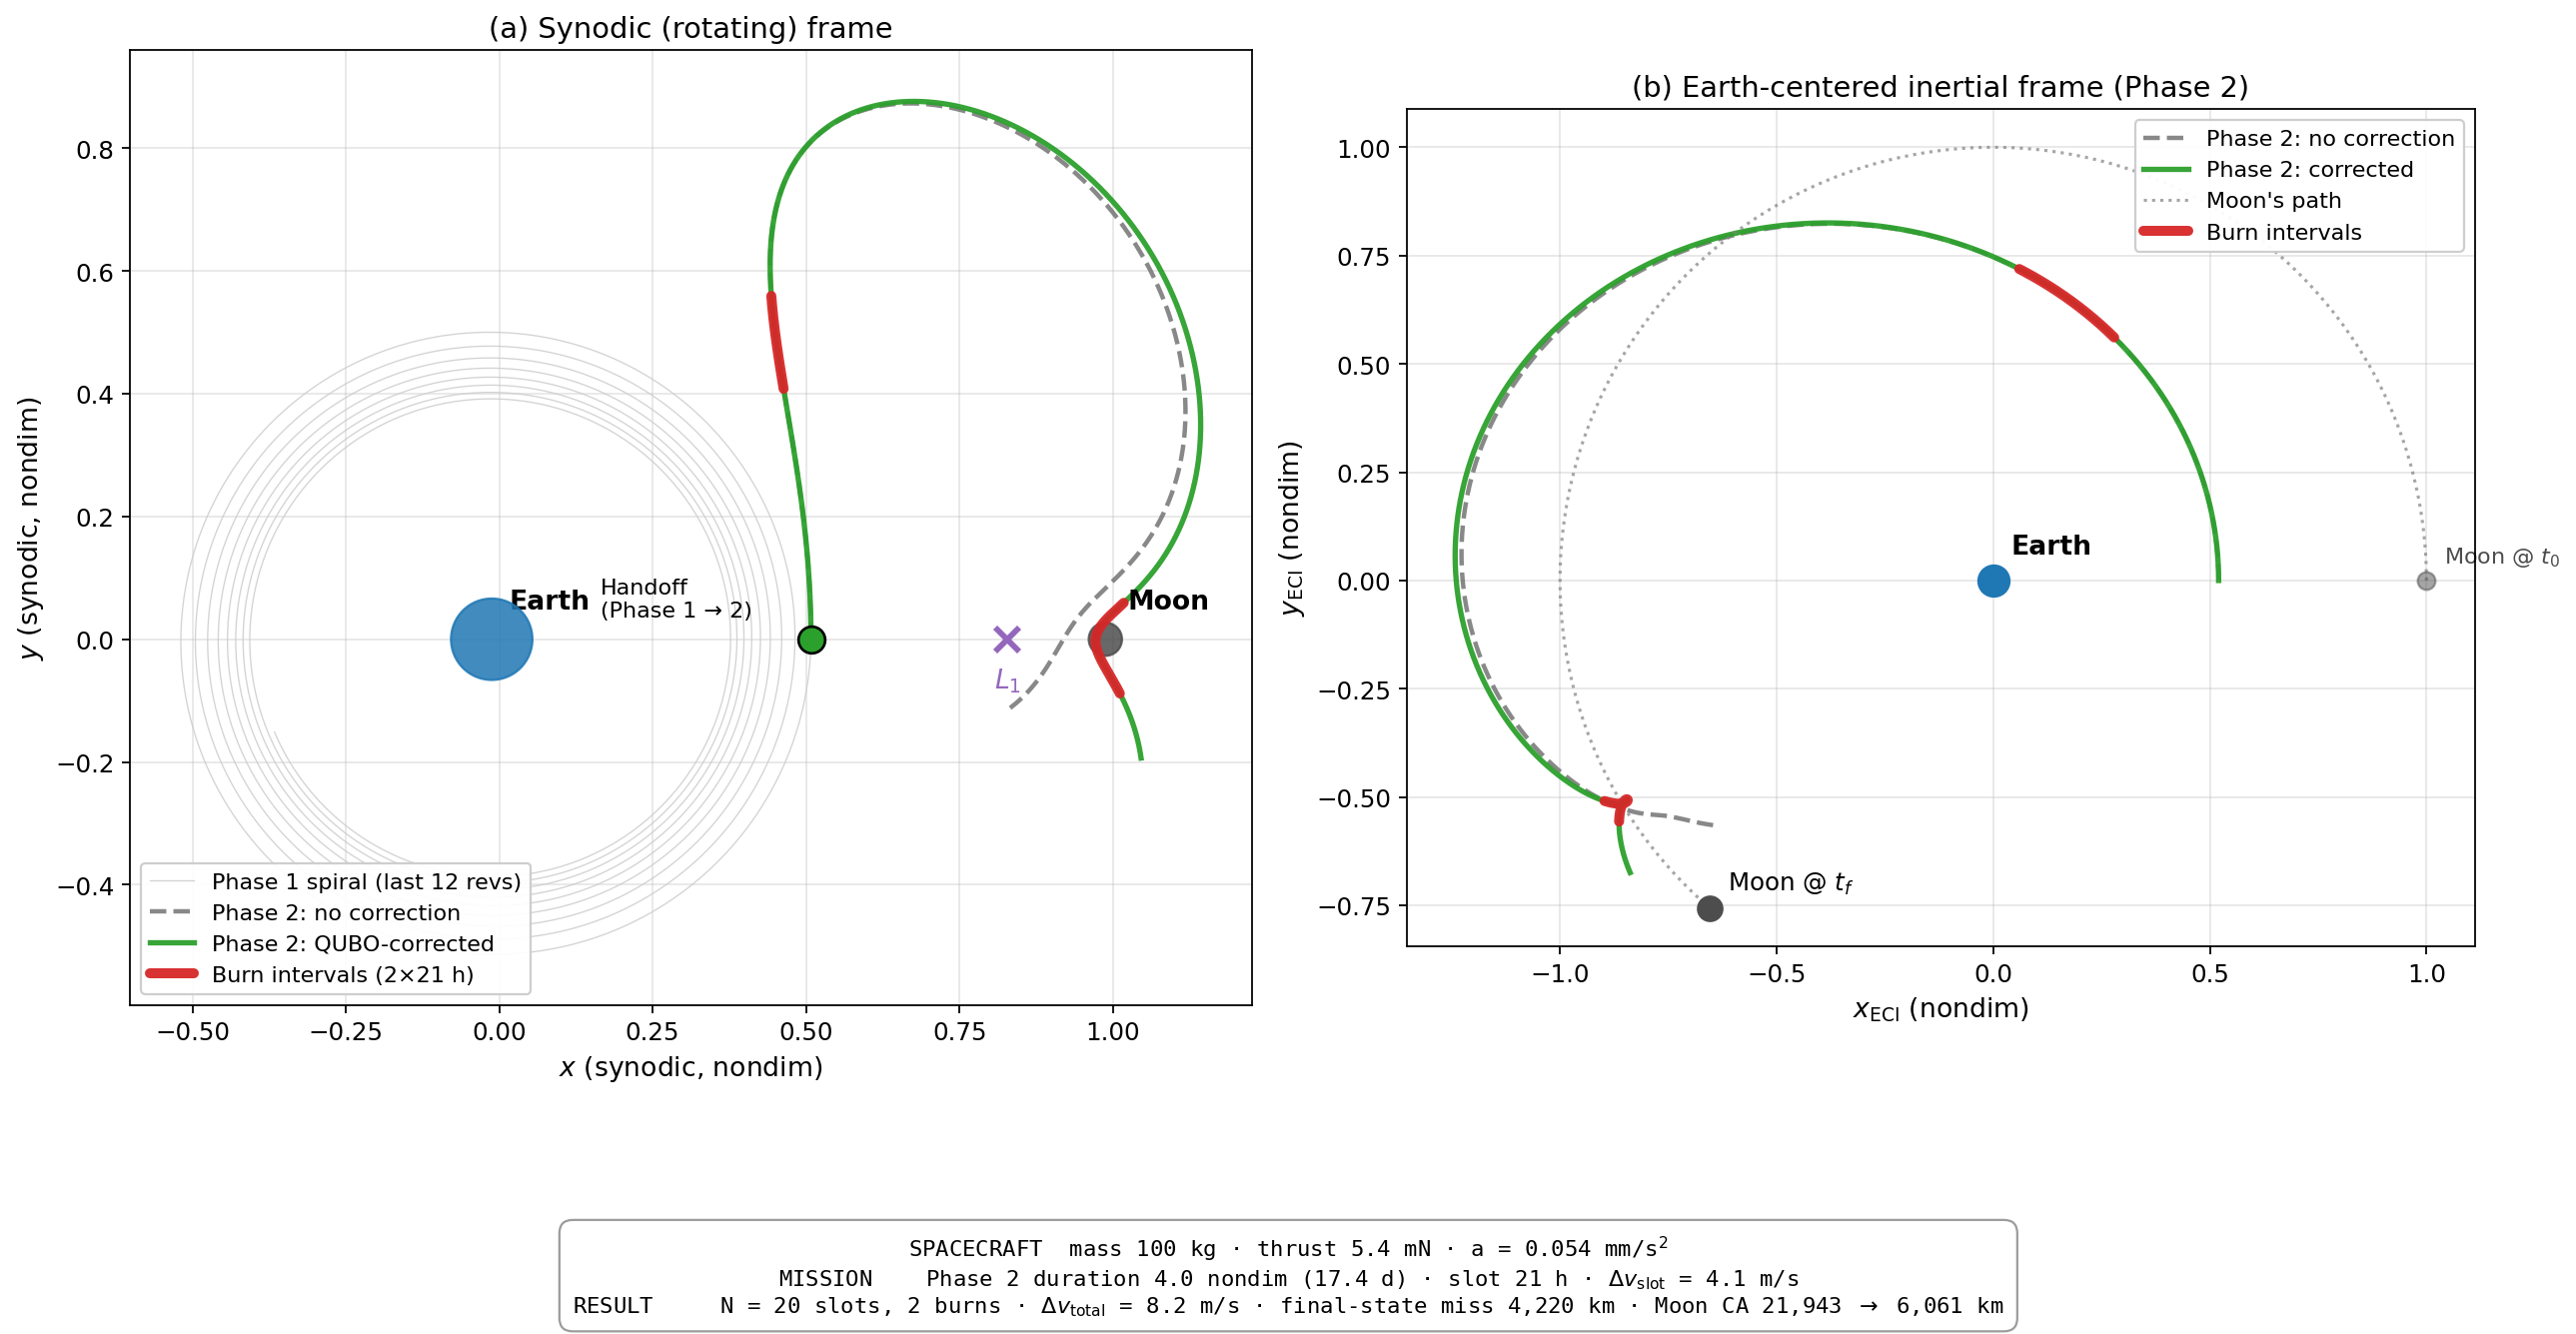
\includegraphics[width=\textwidth]{cislunar_trajectory.png}
\caption{Phase 2 of the mission: cislunar correction trajectory in
two reference frames. (a) CR3BP synodic (rotating) frame: the
last twelve revolutions of the Phase-1 Edelbaum spiral are
visible as light-gray ellipses arriving at the green Handoff
marker; from there the Phase-2 coast (gray dashed) and
QUBO-corrected (green) trajectories diverge toward the Moon,
with the two active burn intervals shown as thick red segments
along the corrected trajectory. (b) Earth-centered inertial
frame, Phase-2 only: the same trajectories appear as a curving
arc over $\sim 17$ days, with the Moon advancing along its
circular path from $t_0$ to $t_f$. The bottom panel summarises
the spacecraft, mission, and result parameters. The thruster
runs in cruise mode for this phase
($a \approx 0.054$~mm/s$^2$, $\sim 5.4$~mN out of the
\SI{350}{\milli\newton} envelope of the throttleable
\SI{100}{\kg} microsatellite). The iterative QUBO selects two
$21$-hour burns for a total $\Delta v$ of $8.2$~m/s, reducing the
lunar closest approach from $\sim 22\,000$~km (coast) to
$\sim 6\,000$~km (corrected).}
\label{fig:trajectory}
\end{figure}

\subsection{Validation: simulated annealing matches brute force}

For $N = 15$ ($2^{15} = 32\,768$ candidate schedules) and at all
multi-channel sizes up to $M = 40$ qubits used in this section, we
solve the QUBO with brute force and with simulated
annealing (\texttt{neal.SimulatedAnnealingSampler}, $1000$--$4000$
reads). Simulated annealing recovers the brute-force optimum on
every problem size where the comparison is computable, so simulated
annealing is a faithful surrogate at this size and a defensible
upstream proxy for quantum-annealing performance.

% ------------------------------------------------------------------
\subsection{Phase 2 demonstration: linearisation gap, single-pass vs
  iterative}\label{sec:lin-gap}
% ------------------------------------------------------------------

This subsection focuses on Phase 2 of the mission introduced in
Sec.~\ref{sec:scenario}: the cislunar trajectory correction at
cruise power. To quantify the value of the iterative
re-linearisation we run a long-arc cislunar correction at $T = 4$
nondim ($\sim 17$ days), $N = 15$,
$v_\mathrm{inj}/v_\mathrm{circ} = 1.187$. At this $T$ the
single-pass linearisation about the coast arc is loose enough that
the QUBO's optimum schedule, when propagated under the true
nonlinear CR3BP, lands far from the target.
Figure~\ref{fig:lin-gap} compares the actual trajectories obtained
from the two solvers on this scenario.

\begin{figure}[h]
\centering
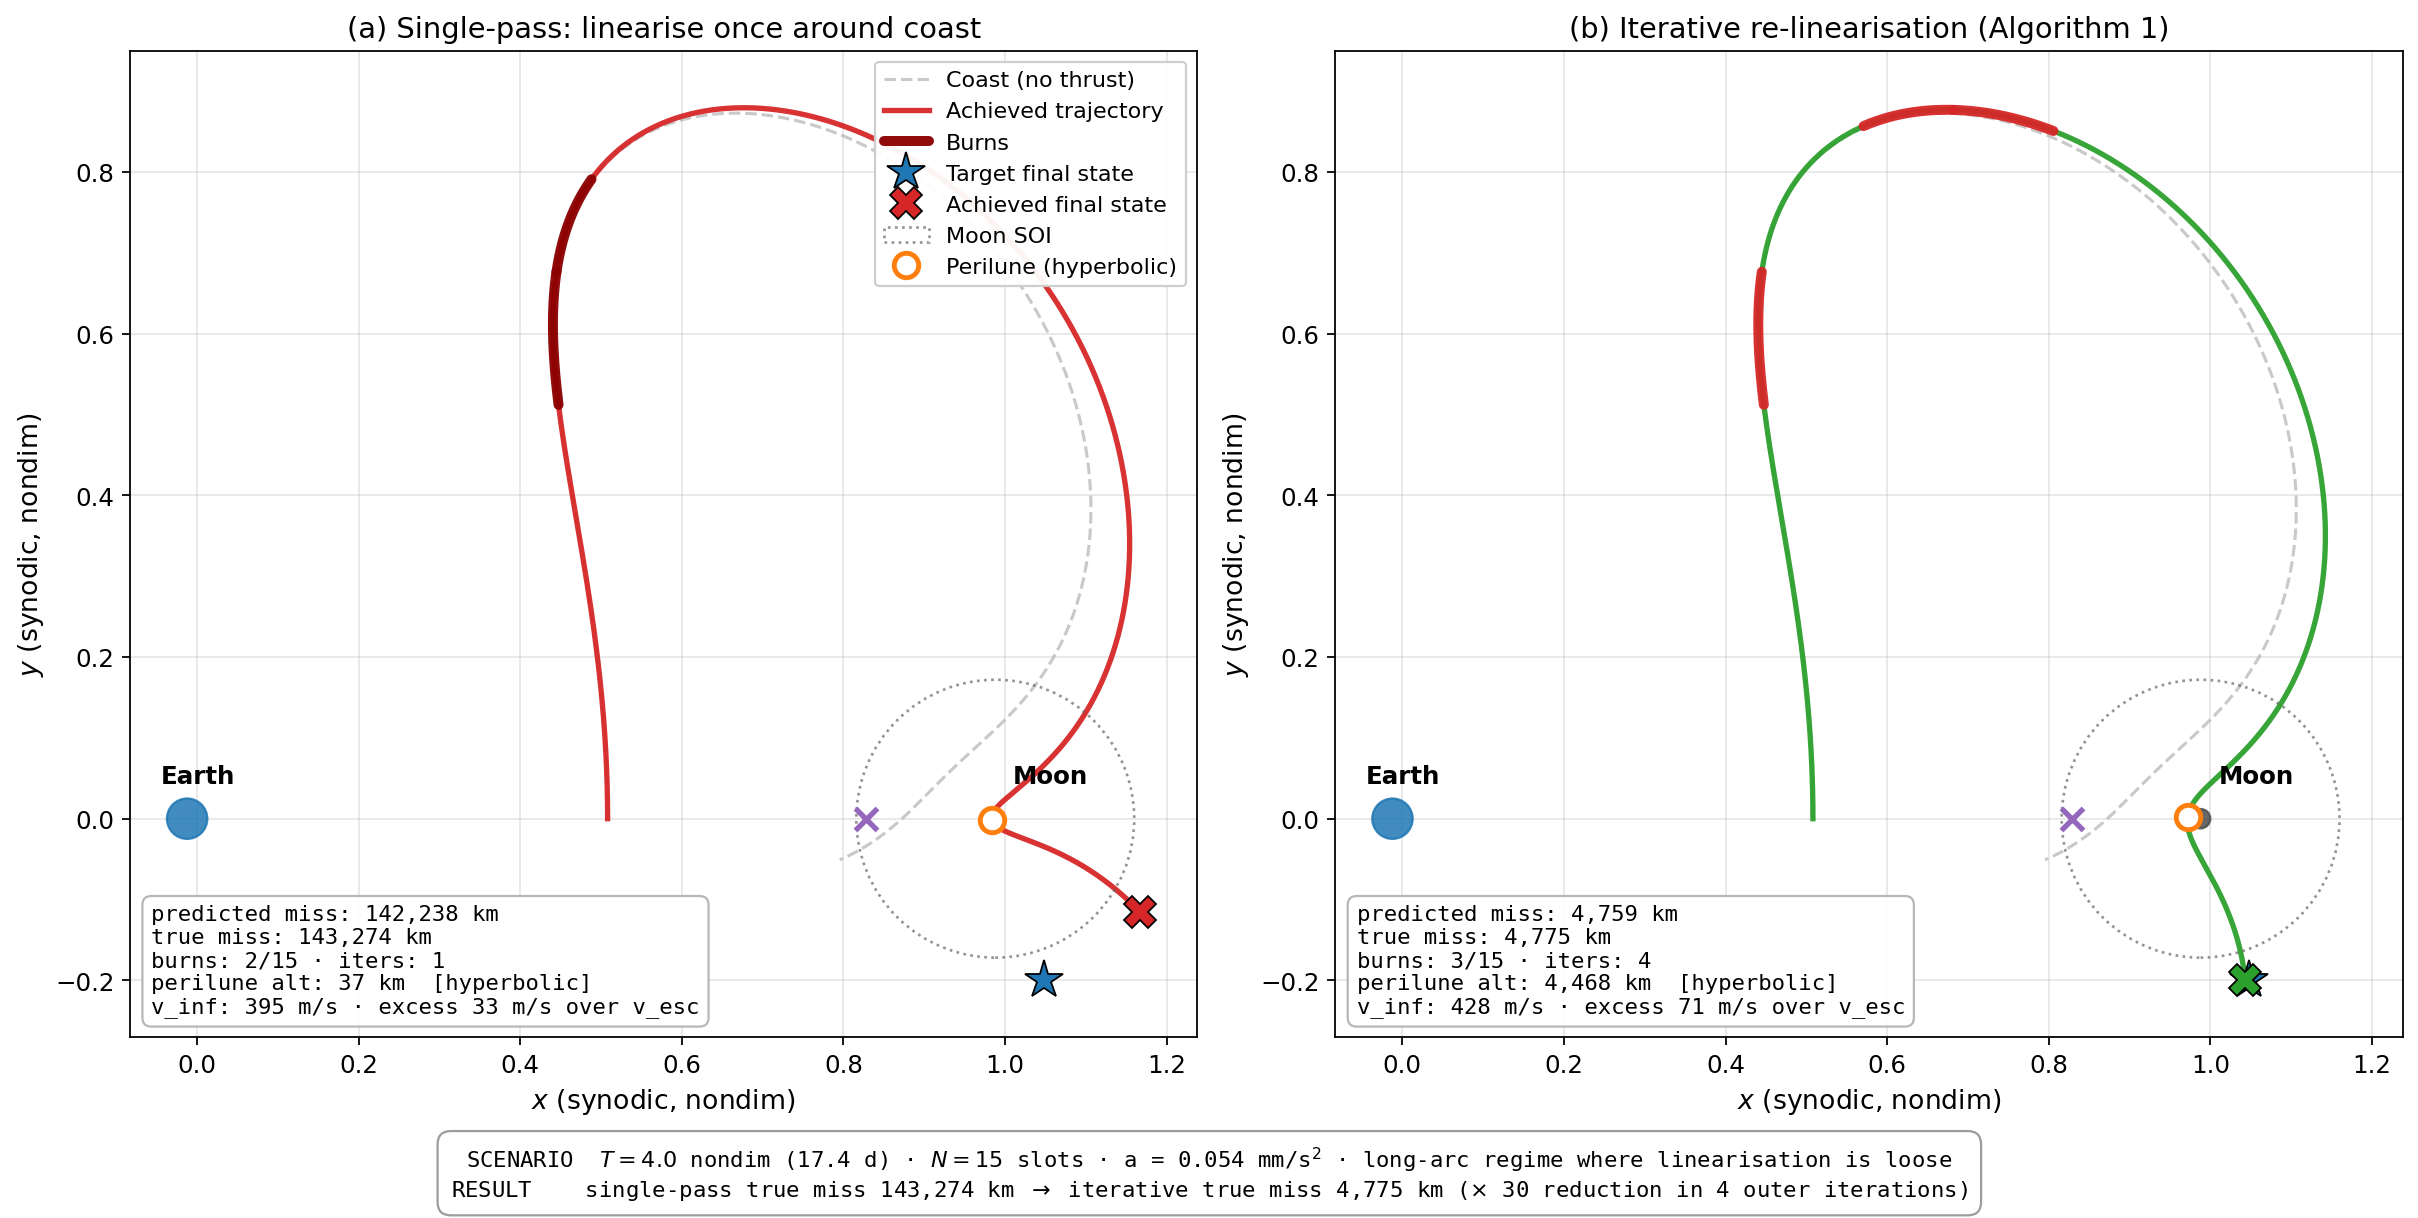
\includegraphics[width=\textwidth]{iterative_vs_singlepass_trajectory.png}
\caption{Single-pass QUBO (a) versus iterative re-linearisation
(b) on a long-arc cislunar correction at $T = 4$ nondim. The blue star is the target final state;
the cross is the achieved final state. The single-pass solver
predicts a $142\,000$~km miss and delivers $143\,000$~km ---
essentially the coast outcome. The iterative solver, after four
outer iterations and three burns, lands within $4\,800$~km of
the target: a $30\times$ reduction in true miss for the cost of
one extra burn. The operational regime of
Phase~2 (Sec.~\ref{sec:end-to-end}) lands the corrected state
within $\sim$$1\,900$~km of the target, inside the Moon SOI,
where the Phase-3 sliding-window scheduler takes over.}
\label{fig:lin-gap}
\end{figure}

The figure shows the operational difference between the two
methods. For the schedule it returns, the single-pass QUBO's
prediction is even accurate ($142\,000$~km predicted,
$143\,000$~km true) --- but that schedule is barely better than
coast. The failure is one of \emph{ranking}: under the coast-arc
linearisation the impulse-response vectors $\bbvec_j$
misrepresent what the genuinely useful schedules would achieve
at $T = 4$, so the QUBO never selects them.
The iterative loop's first outer iteration relinearises around
the single-pass schedule; subsequent iterations refine the
linearisation about progressively closer trajectories until the
QUBO's predicted miss converges to the true nonlinear miss
within numerical tolerance.

Beyond $T \gtrsim 5$ nondim ($\sim 22$ days) the linearisation
gap is so wide that no schedule satisfies the trust-region accept
rule on the first iteration; the loop correctly terminates at
coast.

% ------------------------------------------------------------------
\subsection{Connection to primer-vector
  theory}\label{sec:primer-vector}
% ------------------------------------------------------------------

The on/off scheduling QUBO never computes a Pontryagin costate. Once a schedule has converged under the iterative driver,
however, a costate can be reconstructed \emph{a posteriori} along
the resulting nonlinear trajectory by integrating
\(\dot{\boldsymbol{\lambda}} = -A(\xvec(t))^\top
\boldsymbol{\lambda}\) backward in time from the terminal
transversality condition
\(\boldsymbol{\lambda}(t_f) = 2\Wmat(\xvec_f - \xvec_\mathrm{target})\).
The tangential primer-vector analogue is the scalar switching
function

\begin{equation}
S(t) \;=\; -\boldsymbol{\lambda}_v(t) \cdot \hat{\vvec}(t),
\label{eq:switching}
\end{equation}

where \(\boldsymbol{\lambda}_v\) is the velocity sub-vector of the
costate and \(\hat{\vvec}\) the unit velocity vector. Pontryagin's
minimum principle predicts that the optimal tangential bang-bang
control fires the engine when \(S > 0\) and coasts otherwise.
Comparing this continuous-time prediction with the QUBO's discrete
schedule provides a sanity check on the bridge between the binary
formulation and indirect primer-vector
methods~\cite{Taylor2026}.

Applied to the converged iterative schedule of
Sec.~\ref{sec:lin-gap} ($T = 4$ nondim, $N = 15$, three ON
slots out of fifteen), the reconstruction yields a switching
function \(S(t)\) whose support is a contiguous interval near
the second half of the arc.

This reconstruction is, strictly speaking, a self-consistency
check: \(\boldsymbol{\lambda}\) is built from the QUBO's own
final state and propagated through the QUBO's own trajectory.
A fully external comparison would solve the same problem via
indirect methods (the route taken in~\cite{Taylor2026} via
homotopy continuation in \(\rho\) and \(u_\mathrm{max}\)) and
overlay the two switching functions. We leave that comparison to
future work, as the in-house direct-collocation NLP of
Sec.~\ref{sec:nlp} is energy-optimal rather than fuel-optimal and
therefore lacks a directly comparable primer vector.

% ------------------------------------------------------------------
\subsection{Phase 4 demonstration: lunar-orbit
  station-keeping}\label{sec:moon-orbit}
% ------------------------------------------------------------------

This subsection demonstrates Phase 4 of the mission of
Sec.~\ref{sec:scenario}: long-duration station-keeping at the
operational lunar orbit, run at cruise power
(\SI{5.4}{\milli\newton}, the same operating point as Phase 2
in Sec.~\ref{sec:lin-gap}). The scenario is a $5\,000$-km
circular lunar orbit perturbed by a $0.5\%$ tangential velocity
error at $t_0$, with the iterative QUBO scheduling a single
anti-tangential channel to maintain the orbit against this
perturbation. Over two revolutions ($\sim 28$~hours) the
unperturbed coast trajectory drifts by about $1\,300$~km in
position from the nominal endpoint; the QUBO's $4.4$~m/s
schedule reduces the position miss to $\sim 530$~km, a
$2.4\times$ improvement. Both the coast (gray) and corrected
(green) tracks remain near-circular about the Moon when plotted
in the Moon-relative frame, with the burn intervals appearing
as short red segments distributed across the two revolutions
rather than concentrated at a single anomaly.

The QUBO uses the position-only target-weighting variant
of~\eqref{eq:problem}: a phase shift across the orbit affects the
velocity vector but not the position objective, so a
station-keeping mission that cares about position benefits from the diagonal weight $W = \mathrm{diag}(1,1,0,0)$.
This is a different application of the same method as
Sec.~\ref{sec:lin-gap}, with no changes to the QUBO formulation
or the iterative driver.

This scenario is in the linearisation-faithful regime so the iterative loop
terminates after one outer iteration with the schedule being a
fixed point. The contribution here is not the iteration depth
but the formulation: an on/off binary scheduling problem on a
QUBO solver naturally accommodates the pulse-mode operation of
real spacecraft propulsion, while the trust-region rule keeps
the method robust across thrust regimes.

\subsection{Comparison with continuous-control direct
collocation}\label{sec:nlp}

The standard aerospace-engineering tool for low-thrust trajectory
optimisation is direct collocation NLP --- typically Hermite-Simpson
or Legendre--Gauss--Lobatto with SLSQP /
IPOPT~\cite{Kelly2017,Betts2010}. To position our
QUBO methodology against that benchmark we re-pose the cislunar
correction as an energy-optimal continuous-control problem with
boundary conditions enforced as equalities, and solve it with an
in-house Hermite-Simpson direct-collocation implementation
(40 intervals, SLSQP, $\mathrm{tol} = 10^{-9}$).

\begin{table}[htbp]
\centering
\begin{tabular}{lccrr}
\toprule
Scenario & Method & Miss (km) & $\Delta v$ (m/s) & Solve (s) \\
\midrule
\multirow{2}{*}{$v_\mathrm{inj}/v_\mathrm{circ}=1.187$, $T=2$}
  & QUBO iter.\ ($N{=}15$) & $2\,053$ & $10.9$ & $3.1$ \\
  & NLP HS-direct & $0.0$ & $7.7$ & $1.5$ \\
\multirow{2}{*}{$v_\mathrm{inj}/v_\mathrm{circ}=1.187$, $T=3$}
  & QUBO iter.\ ($N{=}15$) & $1\,087$ & $8.2$ & $4.6$ \\
  & NLP HS-direct & $0.0$ & $8.8$ & $3.2$ \\
\multirow{2}{*}{$v_\mathrm{inj}/v_\mathrm{circ}=1.185$, $T=3$}
  & QUBO iter.\ ($N{=}15$) & $2\,626$ & $20.5$ & $3.4$ \\
  & NLP HS-direct & $0.0$ & $14.6$ & $1.6$ \\
\bottomrule
\end{tabular}
\caption{Iterative QUBO scheduling vs continuous-control direct
collocation NLP on three cislunar correction scenarios. The NLP
enforces final state as an equality constraint and reaches the
target exactly; the QUBO is restricted to a binary tangential
action set and leaves a residual miss of $1\,000$--$2\,600$~km.
The $\Delta v$ cost of the QUBO is comparable but slightly higher
in the strong-error case; solve times are within a factor of two.}
\label{tab:nlp-vs-qubo}
\end{table}

The NLP wins on the standard metric: zero miss at comparable or
lower $\Delta v$. This is expected (it has a richer action
space and explicit BC
satisfaction). The QUBO methodology developed here is appropriate when the
action space is genuinely discrete, a regime in which the
classical NLP is itself not directly applicable without
post-processing.

\paragraph{The continuous ``optimum'' is solver- and
seed-dependent.} A caveat tempers the apparent NLP advantage of
Table~\ref{tab:nlp-vs-qubo}: the Hermite--Simpson transcription of
the energy-optimal CR3BP transfer is a \emph{nonconvex} NLP, so the
``classical optimum'' it returns is not unique --- it depends on
the starting iterate and on the optimiser. We make this explicit
with a multistart study. For three boundary-condition cases we draw
$32$ random seeds (Gaussian perturbations of the
linear-interpolation guess) and solve each from that seed with
SLSQP; we additionally cross-check a subset of the \emph{same} seeds
with MATLAB's \texttt{fmincon} (SQP) on the identical transcription.
Figure~\ref{fig:multistart} reports the result. Almost every
feasible converged solution is a \emph{distinct} local minimum
(case~A: $15$ feasible starts, $15$ distinct minima), and the
objective spans more than an order of magnitude
($J \in [1.41, 19.70]$, a $\sim\!1300\%$ spread). The canonical
linear-interpolation seed lands at $J \approx 4.01$, well above the
multistart best of $J \approx 1.41$. From identical seeds SLSQP and
\texttt{fmincon} descend into different basins in five of six cases,
yet agree to $\sim\!10^{-9}$ whenever they share a basin ---
confirming that the disagreement is genuine nonconvexity of the
problem, not a mismatch between the two transcriptions.

\begin{figure}[htbp]
\centering
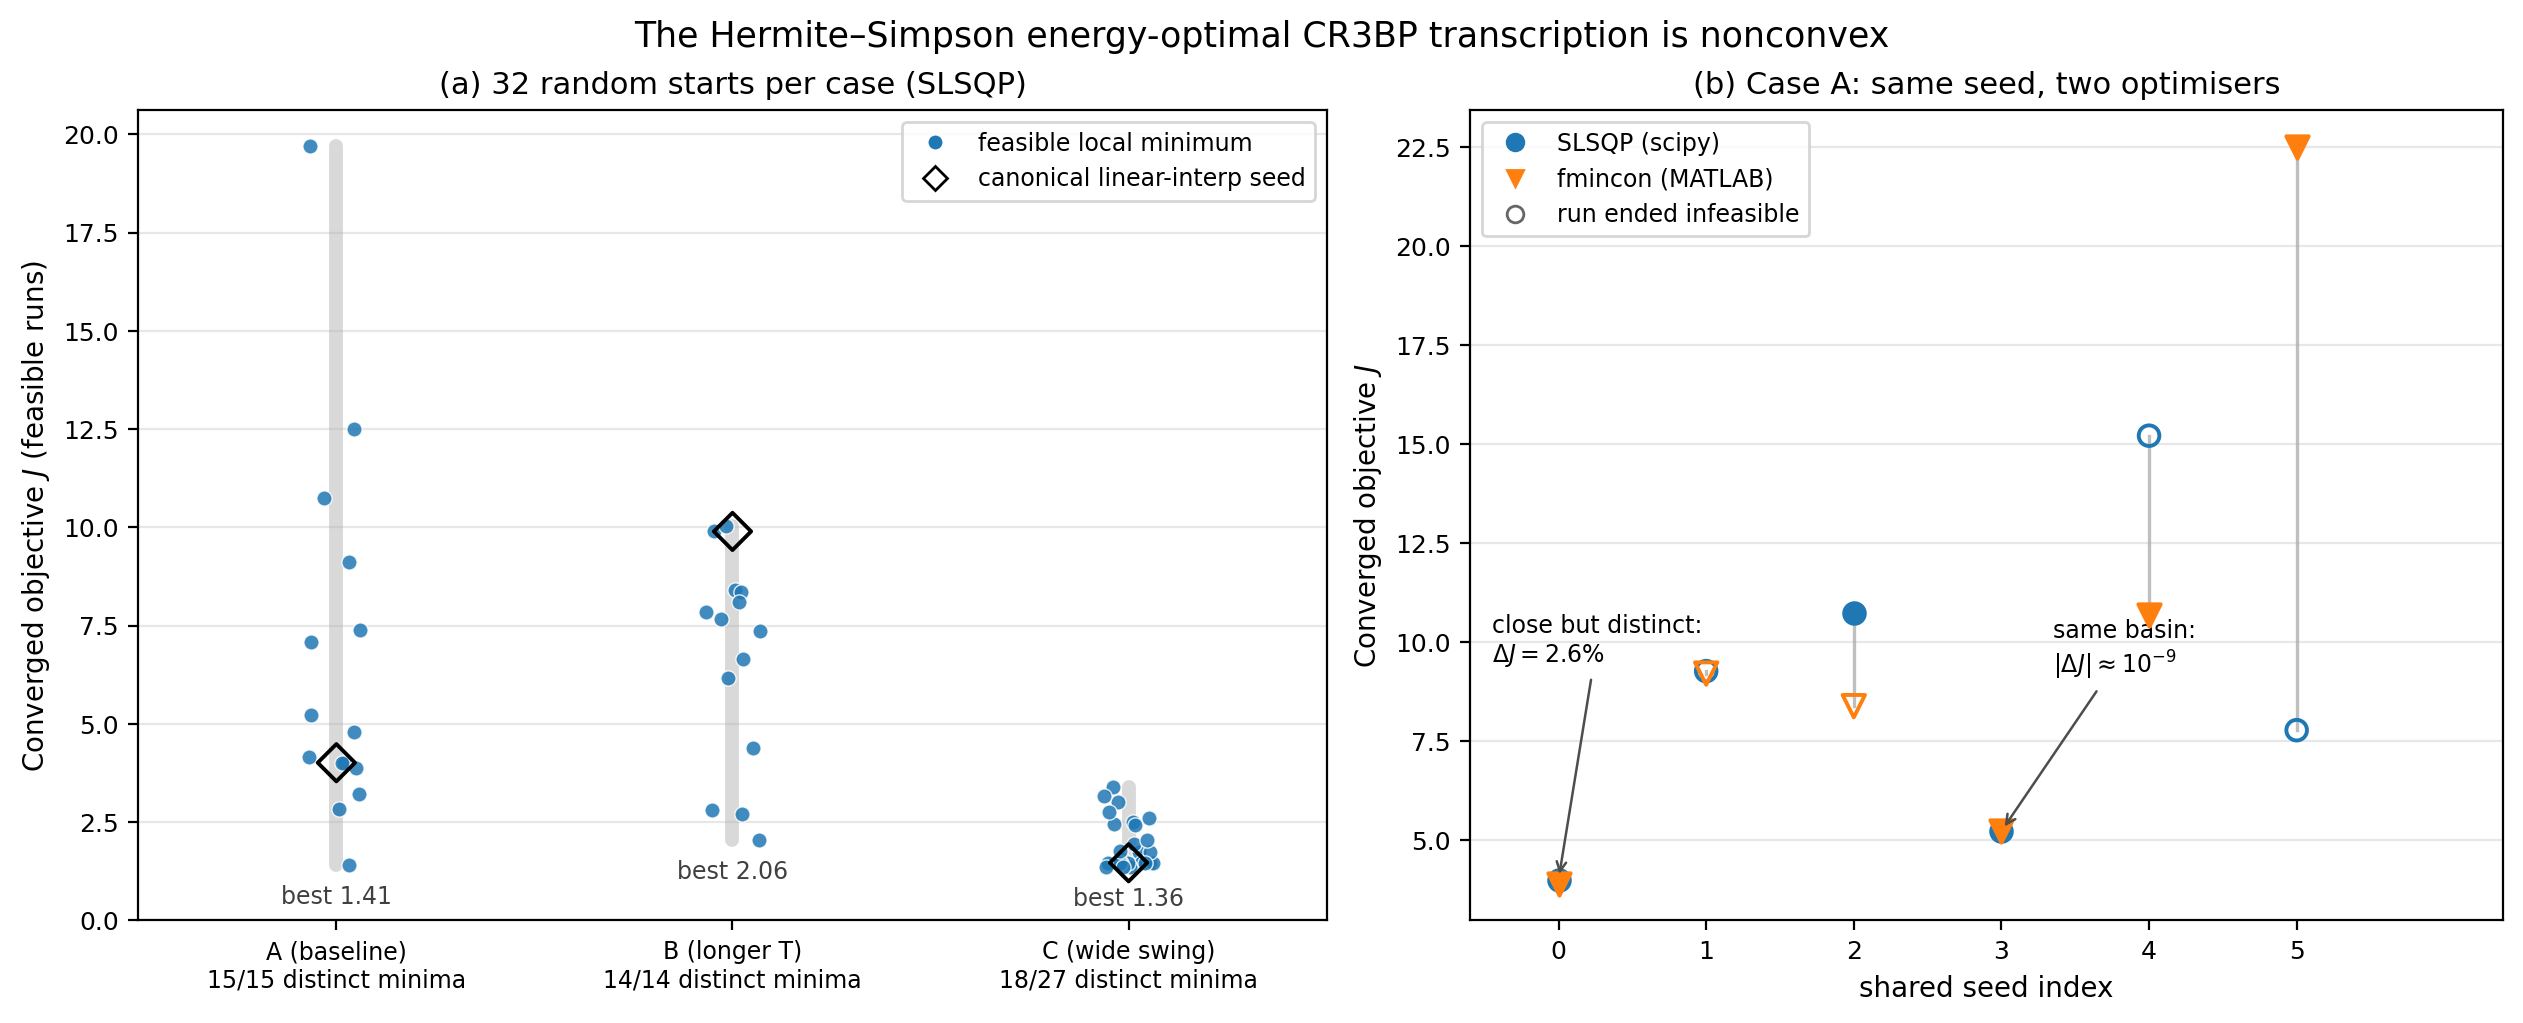
\includegraphics[width=\linewidth]{fmincon_multistart.png}
\caption{The Hermite--Simpson energy-optimal CR3BP transcription is
nonconvex. \emph{(a)}~Feasible converged objectives of $32$ random
multistarts (SLSQP) for three boundary-condition cases: each dot is
one run, the grey bar spans the min--max range, and the open diamond
marks the canonical linear-interpolation seed. The label under each
column counts distinct local minima over feasible runs --- in
case~A every feasible start reaches a \emph{different} minimum, and
the canonical seed ($J \approx 4.01$) sits far above the multistart
best ($J \approx 1.41$). \emph{(b)}~Case~A solved by SLSQP (circles)
and MATLAB \texttt{fmincon} (triangles) from six identical seeds;
open markers are runs that ended infeasible. The optimisers descend
into different basins in five of six seeds, yet agree to
$\sim\!10^{-9}$ in the one shared basin (seed~3) --- the spread is
genuine problem nonconvexity, not a transcription mismatch.}
\label{fig:multistart}
\end{figure}

This does not overturn the comparison of
Table~\ref{tab:nlp-vs-qubo}, but it reframes it: quoting a single
continuous optimum as ``the'' baseline is fragile, and any statement
that the binary QUBO is within $x\%$ of optimal is only as
meaningful as the seed used to compute that baseline. The exact,
seed-independent reference for the binary problem remains the
McCormick-lifted MILP of Sec.~\ref{sec:milp}, which certifies the
global binary optimum; \texttt{fmincon} corroborates the continuous
transcription, and the multistart spread is itself a strong
motivation for the global/combinatorial search that the QUBO
formulation is built to enable.

\subsection{Multi-channel scheduling}\label{sec:multi-channel}

The single-channel formulation restricts thrust to one direction.
Adding channels (anti-tangential, normal, anti-normal) gives the
QUBO direction freedom at the cost of more variables ($M = K N$).
We run the iterative scheduler on three injection-error scenarios
at matched $N = 10$, $T = 3$ nondim, and report the result with
single channel ($K = 1$, $M = 10$) versus four channels
($K = 4$, $M = 40$). Single-channel uses brute force; multi-channel
uses simulated annealing with $4000$ reads.

\begin{table}[htbp]
\centering
\begin{tabular}{lcrrr}
\toprule
Scenario & Mode & Miss (km) & $\Delta v$ (m/s) & Burns \\
\midrule
\multirow{2}{*}{Speed-only}
  & tangential ($M{=}10$) & $3\,729$ & $24.6$ & $4$ \\
  & 4-channel ($M{=}40$) & $880$ & $153.5$ & $25$ \\
\multirow{2}{*}{Mixed}
  & tangential ($M{=}10$) & $2\,950$ & $18.4$ & $3$ \\
  & 4-channel ($M{=}40$) & $1\,624$ & $165.8$ & $27$ \\
\bottomrule
\end{tabular}
\caption{Multi-channel vs single-channel iterative scheduling at
$T = 3$ nondim, $a = 0.02$, $N = 10$. The 4-channel mode adds
anti-tangential, normal, and anti-normal directions. It reduces
miss by a factor of $\sim 4$ on the speed-error scenario and
$\sim 1.8$ on the mixed scenario, at a substantially higher
$\Delta v$.}
\label{tab:multi-channel}
\end{table}

The speed-error and mixed scenarios show the expected pattern:
extra direction freedom permits substantially smaller miss when
the gap is not aligned with the spacecraft velocity. The
$\Delta v$ cost rises roughly linearly with the number of active
burns (each burn fires one engine for $\Delta t$ at acceleration
$a$), so the methodology trades fuel for accuracy in the natural
way. 

\subsection{Scaling}\label{sec:scaling}

We measured solve times and best
energies for brute force, McCormick-lifted MILP via HiGHS,
simulated annealing, and the local Kerberos workflow from
\texttt{dwave-hybrid} on the cislunar scenario at increasing $N$.
All four solvers operate on the identical QUBO. Brute force is
the optimal-by-construction reference at $N \le 20$.

Three operational regimes emerge from the data. For $N \le 20$
all four solvers find the global optimum and selection is purely
on speed (SA fastest, brute force slowest). For $20 < N \lesssim
50$ MILP can no longer certify optimality but the LP relaxation
is still tight enough that the incumbent is competitive with
SA. For $N \gtrsim 100$ MILP collapses (the dense $\Qmat$ makes
the relaxation order-of-magnitude loose) and the choice is
between the SA heuristic and the hybrid Kerberos workflow.
Kerberos in this regime returns lower-energy solutions than
SA in significantly less time, consistent with the design
intent of \texttt{dwave-hybrid}~\cite{DWave2024}, which
decomposes the problem and runs classical heuristics on the
parts in parallel.

The scientifically relevant claim is therefore not that quantum
annealing offers an asymptotic speedup over classical brute force, but that the hybrid workflow architecture can
match or beat raw simulated annealing at large $N$. A direct
submission of the same QUBO to a Leap Hybrid solver (or to an
Advantage~2 QPU when access is available) is the natural
extension of this comparison and is implemented behind the
sampler interface in the accompanying code.

% ------------------------------------------------------------------
\subsection{End-to-end mission: composing Phases 1, 2 and
  3}\label{sec:end-to-end}
% ------------------------------------------------------------------

The previous subsections demonstrated each phase of the mission of
Sec.~\ref{sec:scenario} in isolation: Phase 2 cislunar correction
in Sec.~\ref{sec:lin-gap}, Phase 4 station-keeping in
Sec.~\ref{sec:moon-orbit}. We now compose Phases 1, 2, and 3 into a
single end-to-end Earth-to-bound-lunar-orbit transfer flown by the
same spacecraft and the same throttleable thruster, with no
impulsive burns.

\paragraph{Mission totals.} Table~\ref{tab:end-to-end} summarises
the breakdown. The complete mission delivers
$\Delta v_\mathrm{total} \approx
 \SI{2502}{\meter\per\second}$ in
\SI{31.8}{\day} of flight, with every metre per second produced
by binary on/off commands of a single thruster.

\begin{table}[h]
\centering
\caption{All-binary Earth--Moon mission breakdown.}
\label{tab:end-to-end}
\begin{tabular}{lrrl}
\toprule
Phase & $\Delta v$ (m/s) & TOF (days) & Mode \\
\midrule
1: Edelbaum spiral + injection boost
  & \num{1924} & \num{6.4} & main, tangential \\
2: cislunar correction (QUBO)
  & \num{16}   & \num{17.4} & cruise, tangential \\
3: sliding-window QUBO capture
  & \num{561}  & \num{8.0}  & main, anti-tangential \\
\midrule
Total
  & \num{2502} & \num{31.8} & all binary \\
\bottomrule
\end{tabular}
\end{table}

Figure~\ref{fig:mission-overview} shows the three-panel mission
diagram. Phase~1 dominates the $\Delta v$ budget at
\SI{1924}{\meter\per\second} (\(77\%\) of the total), Phase~3 is
the second-largest cost at \SI{561}{\meter\per\second}
(\(22\%\)), and Phase~2 contributes \SI{16}{\meter\per\second}
(\(0.6\%\)), essentially free in comparison; yet without the
Phase-2 correction the \num{22000}-km miss precludes any usable
perilune passage and the mission cannot continue.

\begin{figure}[h]
\centering
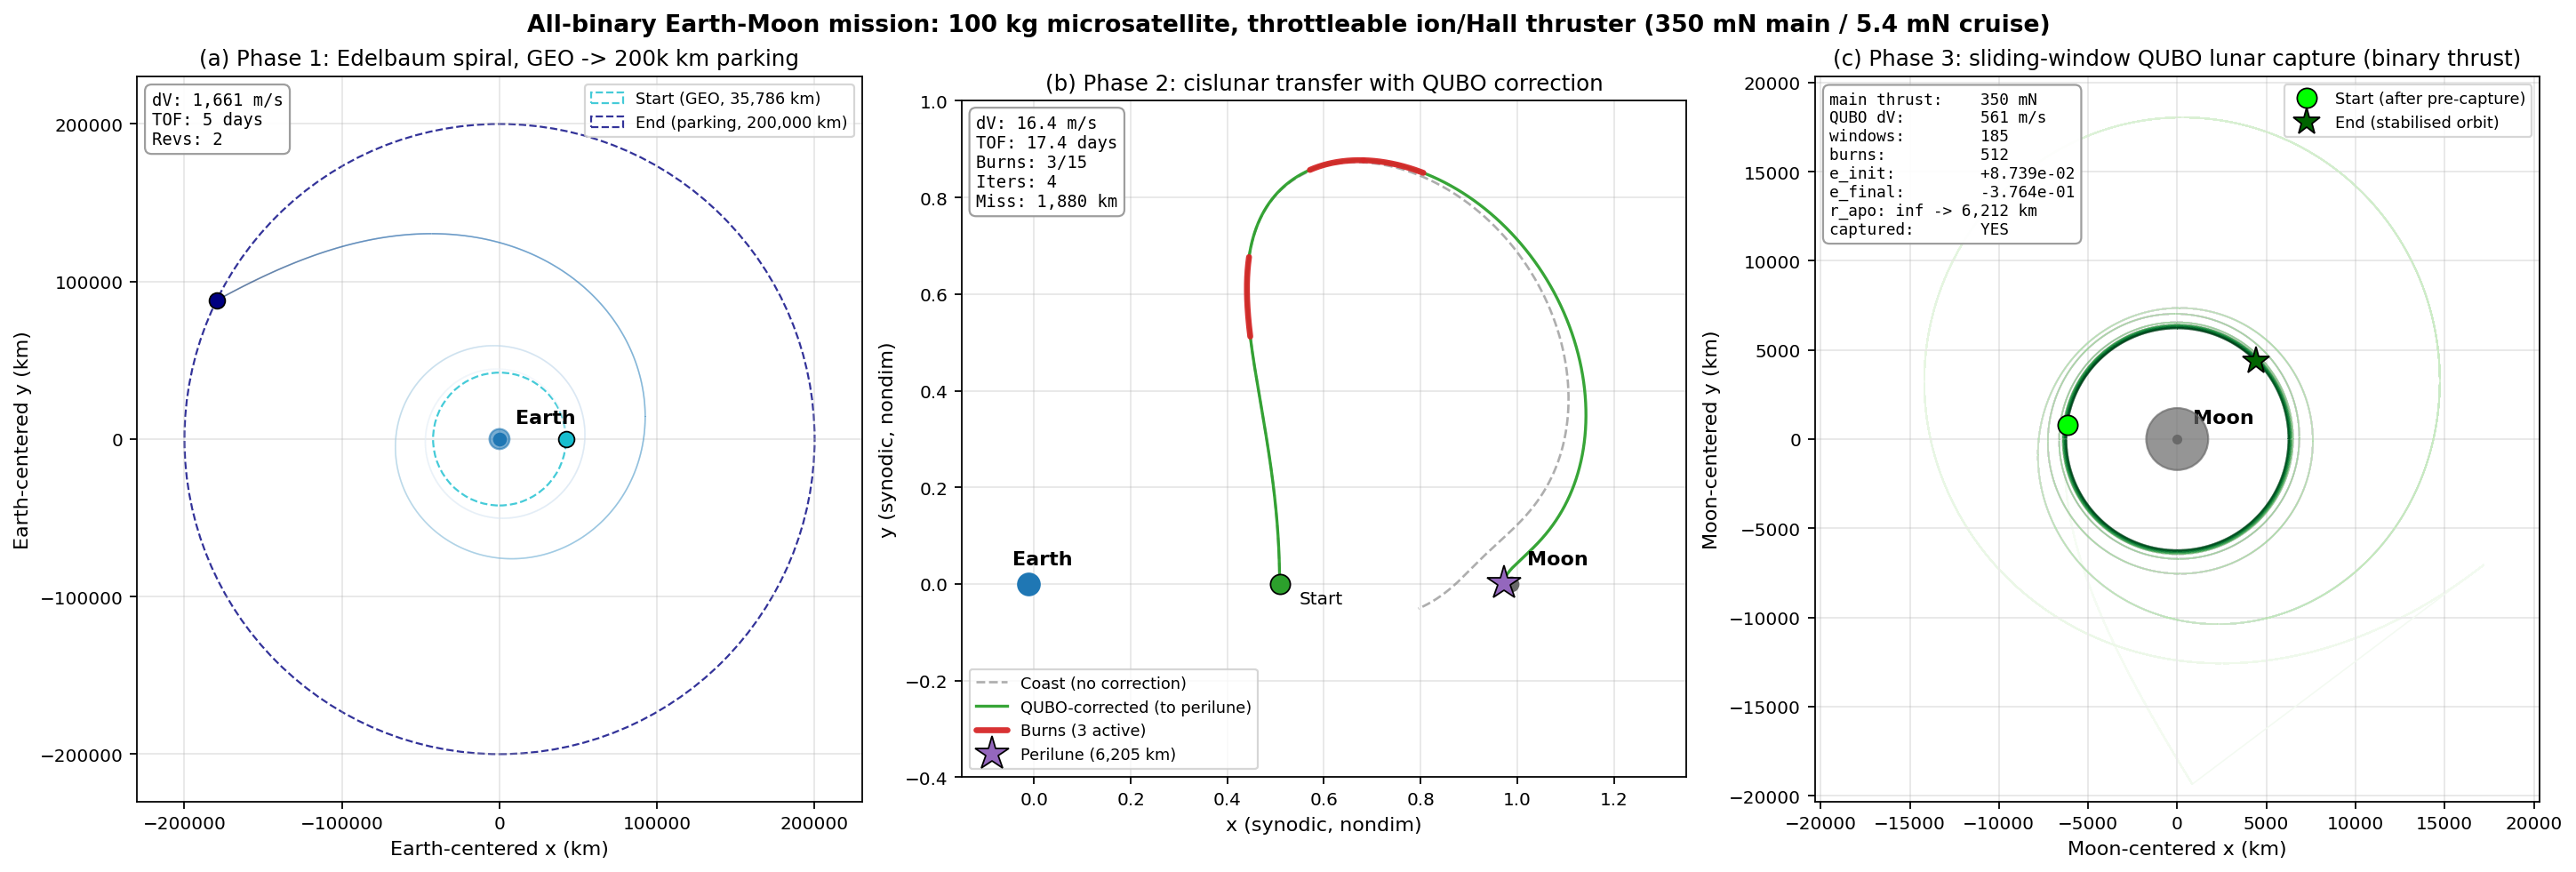
\includegraphics[width=1\linewidth]{mission_overview.png}
\caption{All-binary Earth--Moon mission overview.
(a) Phase~1 Edelbaum spiral from GEO to a \SI{200000}{\km}
parking orbit, Earth-centered. (b) Phase~2 cislunar transfer
under iterative-QUBO correction in the synodic frame; coast
(grey dashed) drifts to a \SI{22000}{\km} miss while the QUBO
corrects to \SI{1880}{\km} miss with three burns.
(c) Phase~3 sliding-window QUBO capture trajectory in the
Moon-relative frame; the spacecraft enters hyperbolic from
Phase~2 and is brought into a bound, near-circular orbit by
binary anti-tangential pulses during $\sim$\num{200} short
windows. The $\Delta v$ breakdown and TOF totals are reported
in Table~\ref{tab:end-to-end}.}
\label{fig:mission-overview}
\end{figure}

The three-panel overview of
Figure~\ref{fig:mission-overview} plots each phase in the frame
that is most natural for it (Earth-inertial for Phase~1, synodic
for Phase~2 and~3), which can hide the fact that the trajectory
is physically continuous. Figure~\ref{fig:mission-continuity} makes that
continuity explicit. 

\begin{figure}[h]
\centering
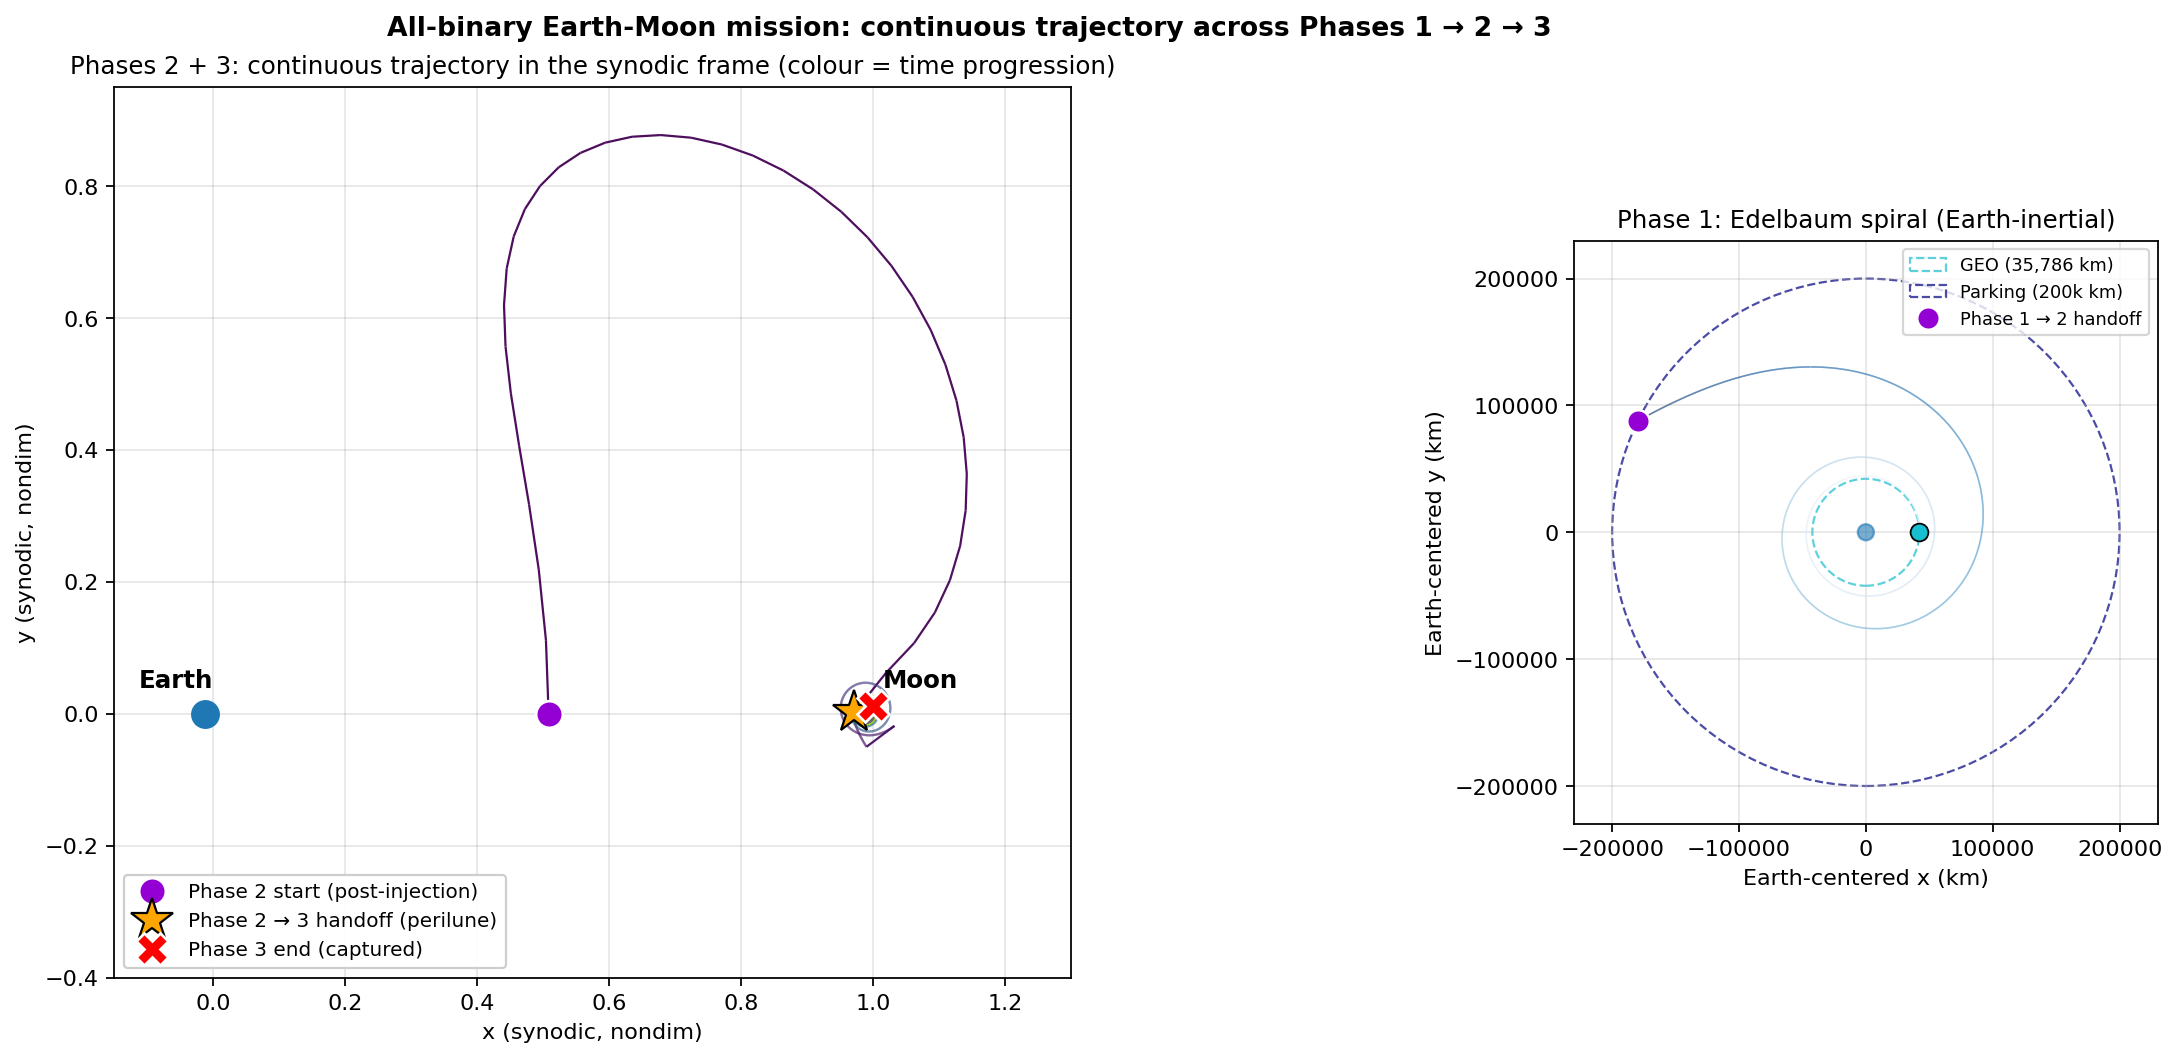
\includegraphics[width=0.98\linewidth]{mission_continuity.png}
\caption{Continuity of the all-binary mission across
Phases~1\,$\to$\,2\,$\to$\,3.
\emph{Left:} Phases~2 and~3 plotted as a single continuous
trajectory in the synodic frame, with a viridis colour gradient
encoding mission elapsed time; the orange star marks the
Phase~2\,$\to$\,3 handoff at perilune, which lies on the curve
rather than separating two distinct curves.
\emph{Right:} Phase~1 in Earth-inertial coordinates with the
GEO start and parking-orbit end circles; the handoff marker
identifies the state that becomes the Phase-2 initial condition.
The cumulative $\Delta v$ and altitude histories are described
in the surrounding text.}
\label{fig:mission-continuity}
\end{figure}

\paragraph{Validation against flown missions.} To place the
all-binary budget of Table~\ref{tab:end-to-end} in context, we
compare it with three flown Earth--Moon missions spanning the
propulsion regimes (Fig.~\ref{fig:benchmark}). The apples-to-apples
reference is ESA's SMART-1, the canonical solar-electric low-thrust
spiral to the Moon: it delivered $\approx\SI{3.5}{\km\per\second}$
over $\sim\!13$ months from a GTO start with a \SI{70}{\milli\newton}
Hall thruster~\cite{Racca2002,Milligan2005}. Our mission's
$\SI{2502}{\meter\per\second}$ sits in the same electric-propulsion
band, and its propellant fraction at a comparable specific impulse
($I_\mathrm{sp}\approx\SI{1640}{\second}$) is $\approx\!14\%$ against
SMART-1's $\approx\!20\%$. Two caveats keep the comparison honest.
First, our spiral departs a \emph{circular} GEO whereas SMART-1
departed a GTO with a low perigee, which accounts for part of the
lower Phase-1 cost. Second, and dominant, our assumed initial
acceleration $a_0 = \SI{3.5}{\milli\meter\per\second\squared}$ is
roughly $18\times$ SMART-1's
$\SI{0.19}{\milli\meter\per\second\squared}$; this --- not any
property of the scheduling --- is why the present time of flight is
$\sim\!1$~month against SMART-1's $\sim\!13$, and it is an optimistic
high-power assumption for a \SI{100}{\kg} bus.

To remove that confound entirely we re-run the \emph{same} analytical
Edelbaum spiral at SMART-1's own operating point: $a_0 =
\SI{0.19}{\milli\meter\per\second\squared}$, $I_\mathrm{sp} =
\SI{1640}{\second}$, and a circular start orbit carrying SMART-1's
GTO energy (semi-major axis $a_\mathrm{GTO} \approx \SI{24629}{\km}$).
Because the Edelbaum $\Delta v$ depends only on the start/end circular
speeds and not on thrust, while the time of flight scales as $\Delta v
/ a_0$, this is a parameter-matched like-for-like check. The spiral to
the Moon's sphere of influence then costs $\approx\SI{2.9}{\km\per\second}$
over $136$ revolutions, and at SMART-1's $\sim\!40\%$ thrust duty cycle
takes $\approx\!440$~days --- against SMART-1's flown
$\SI{3.5}{\km\per\second}$ (which additionally includes lunar capture),
$207$ revolutions, and $\sim\!410$~days. The agreement in $\Delta v$
magnitude, revolution count, and duty-adjusted time of flight (the
second qalunar marker in Fig.~\ref{fig:benchmark}, which falls on
SMART-1) confirms that the earlier $\sim\!1$-month figure reflected the
$18\times$ higher thrust-to-mass of the demonstrator spacecraft, not
any discrepancy in the transfer physics. The point is therefore not
that the binary mission is cheaper, but that its end-to-end budget is
physically consistent with flown electric-propulsion practice once the
operating point is matched. CAPSTONE's low-energy ballistic transfer
and Apollo's impulsive chemical transfer bracket the other two regimes
in Fig.~\ref{fig:benchmark}.

\begin{figure}[h]
\centering
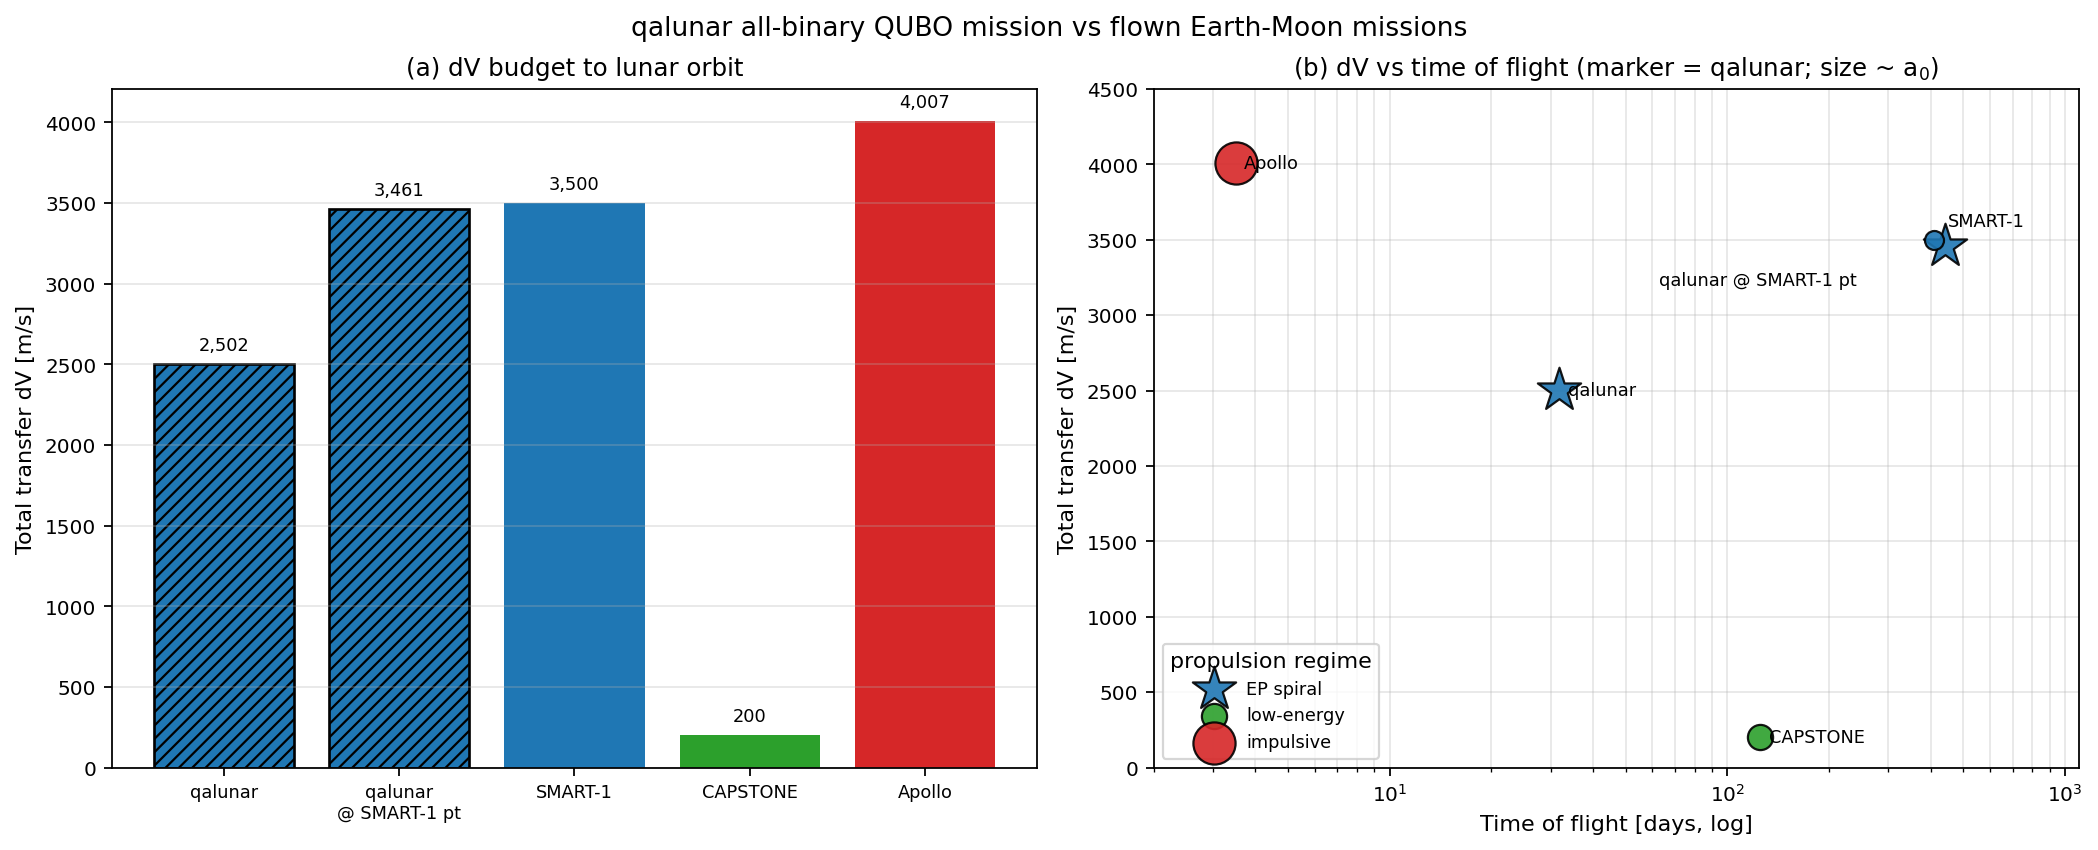
\includegraphics[width=\linewidth]{mission_benchmark.png}
\caption{The all-binary mission against flown Earth--Moon missions.
\emph{Left:} total transfer $\Delta v$ to lunar orbit; the hatched
bars are this work. \emph{Right:} $\Delta v$ versus time of flight
(log scale), coloured by propulsion regime and sized by initial
thrust-to-mass $a_0$. The two qalunar markers (stars) are the
demonstrator end-to-end mission of Table~\ref{tab:end-to-end}
($a_0 = \SI{3.5}{\milli\meter\per\second\squared}$, $\sim\!1$ month)
and the \emph{same} spiral re-run at SMART-1's operating point
($a_0 = \SI{0.19}{\milli\meter\per\second\squared}$, GTO-energy
start, $\sim\!40\%$ duty), which falls on SMART-1. Figures for
SMART-1, CAPSTONE, and Apollo are published values (see text).}
\label{fig:benchmark}
\end{figure}

% ==================================================================
\section{Discussion}\label{sec:discussion}
% ==================================================================

\paragraph{When to use which QUBO formulation.} The naturally-binary formulation is the
natural fit when the engine is pulse-driven, when the mission
constraints favour a finite list of discrete burn slots, or when
the linearisation about a reference trajectory is faithful enough
that the squared-norm objective is a good proxy for the true miss.
For the Earth--Moon injection-correction scenario considered here,
the linearisation around the unforced coast arc has three regimes
that the experiments of Sec.~\ref{sec:results} delineate: a
\emph{single-pass-faithful} regime ($T \lesssim 2.5$ nondim,
$\sim$\SI{11}{\day}, where one linearisation suffices), an
\emph{iterative} regime ($2.5 \lesssim T \lesssim 5$, where
Algorithm~1 closes the gap in a few outer iterations), and an
\emph{abstention} regime ($T \gtrsim 5$, where the trust-region
rule rejects every candidate and the method falls back to coast
rather than return a misleading schedule).

\paragraph{Trust-region rule as the operational difference.}
Single-pass QUBO solves are routinely reported in the QA literature
without a trust-region accept rule, on the implicit assumption that
the linearisation is faithful. Our experiments show this assumption
holds only inside the single-pass-faithful regime
($T \lesssim 2.5$ nondim, $\sim 11$~days); beyond it, an unguarded
single-pass can recommend a schedule that is worse than coast.
The accept-or-reject rule of Algorithm~1 is the
binary analogue of a trust-region method in continuous nonlinear
optimisation~\cite{Conn2000}; we recommend that any QUBO-based trajectory tool
adopt it as a default.

\paragraph{From single-arc QUBO to a complete binary mission.}
The end-to-end demo of Sec.~\ref{sec:end-to-end} shows that
the same scheduling formulation, applied window by window,
extends from a single trajectory correction to an entire
Earth--Moon transfer with no impulsive burns.

\paragraph{Comparison with state-of-the-art Earth--Moon
transfers.} Recent work by Taylor et~al.~\cite{Taylor2026} from
the Purdue Orbital student team designs Earth-to-NRHO and
Earth-to-LLO transfers via Pontryagin's Minimum Principle and
primer vector (PV) theory, with hyperbolic-tangent smoothing and
homotopy continuation in $\rho$ and $u_\mathrm{max}$ to converge
on the impulsive limit. Their reported totals are
\SI{3.93}{\km\per\second} in \SI{5.2}{\day} for LEO\,$\to$\,NRHO
and \SI{3.91}{\km\per\second} in \SI{4.7}{\day} for
LEO\,$\to$\,LLO. Table~\ref{tab:purdue-comparison} places those
numbers next to our end-to-end binary-QUBO result. The comparison
is not apples-to-apples in three respects: (i)~the starting orbit
differs (GEO vs.\ LEO; a $\sim$\SI{3.9}{\km\per\second} Hohmann
gap that favours qalunar), (ii)~the propulsion system differs, and (iii)~the final
orbit differs (qalunar reaches a near-circular bound orbit at the
perilune radius rather than \SI{100}{\km} LLO or the 9{:}2 NRHO).
Subject to those caveats, the qualitative conclusion is that the
binary-QUBO formulation produces a $\Delta v$ budget consistent
with the indirect-method state of the art at the cost of an order
of magnitude longer TOF (the expected low-thrust trade-off). The
methodological novelty here is not a $\Delta v$ improvement but
the demonstration that an entire Earth--Moon mission can be flown
by binary on/off commands of a single throttleable thruster, with
the QUBO scheduler and its sliding-window extension as the
discrete-side analogue of the indirect primer-vector switching
function~\cite{Taylor2026}.

\begin{table}[htbp]
\centering
\caption{End-to-end Earth--Moon transfer comparison. The
\emph{Method} column lists the principal optimisation framework;
totals are not directly comparable due to differences in starting
orbit, propulsion system, and final orbit (see text).}
\label{tab:purdue-comparison}
\begin{tabular}{llrrl}
\toprule
Source & Transfer & $\Delta v$ (km/s) & TOF (d) & Method \\
\midrule
This work
  & GEO\,$\to$\,bound lunar orbit
  & \num{2.50} & \num{31.8}
  & binary QUBO, low-thrust \\
\cite{Taylor2026}
  & LEO\,$\to$\,9{:}2 NRHO
  & \num{3.93} & \num{5.2}
  & PMP + PV, impulsive \\
\cite{Taylor2026}
  & LEO\,$\to$\,LLO (\SI{100}{\km})
  & \num{3.91} & \num{4.7}
  & PMP + PV, impulsive \\
\bottomrule
\end{tabular}
\end{table}

\paragraph{Limitations and future work.} The present results use
classical samplers as upstream proxies for quantum
annealing. The extension to D-Wave Leap Hybrid (BQM and
nonlinear) and to direct submission of the QUBO to the
Advantage 2 quantum processor is a natural next step and is
implemented behind a sampler interface in the accompanying code.
Reporting hardware results is left to a follow-up.
The single-channel formulation restricts the action set; a
multi-channel run with simultaneous tangential, normal, and
binormal axes is supported by the code but not yet swept
parametrically. Beyond the planar problem, the same
formulation extends to the full spatial CR3BP with an 8-state
phase space and three thrust channels at the cost of a larger
QUBO, but no qualitative changes to the methodology.

The all-binary mission of Sec.~\ref{sec:end-to-end} reaches a
near-circular bound orbit at the perilune radius
($\sim$\SI{4500}{\km} altitude). A more interesting
extension is a fully four-body model (Earth--Moon--Sun) that
admits weak-stability-boundary trajectories in which the
Moon-relative perilune speed approaches escape velocity
naturally; in that regime the energy budget for binary capture
collapses to a few metres per second and the throttling
asymmetry between Phases~2 and~3 disappears. Finally, the
sliding-window structure is currently parameter-agnostic: an
adaptive choice of window length, action radius, and
brake-factor based on the running orbital state would close
the loop with an autonomous capture controller.

% ==================================================================
\section{Conclusion}\label{sec:conclusion}
% ==================================================================

We presented a naturally-binary QUBO formulation of low-thrust
cislunar trajectory scheduling in the planar CR3BP, complementary
to the continuous-coefficient QUBO formulation of De Grossi,
Carbone et~al. The binary decision variables avoid the
quantisation floor that plagues the continuous formulation, and
the per-step on/off semantics matches both the physical engine
operation and the quantum-annealing variable space. A
sequential re-linearisation outer loop with a trust-region
accept rule closes the linearisation gap on long arcs and
abstains outside its basin of attraction, properties the
single-pass solve does not have. Classical baselines via
McCormick-lifted MILP certify optimality up to
$N \approx 20$, and the SA-vs-MILP scaling crossover near
$N \approx 25$--$30$ delineates the regime where moving to
D-Wave hardware becomes quantitatively defensible.

A sliding-window extension of the iterative driver chains short
single-arc QUBOs across many lunar revolutions and, paired with
an action-radius gate and a velocity-only circular target,
captures a hyperbolic flyby into a bound near-circular orbit
under purely binary anti-tangential thrust. We use it together
with the original cislunar-correction QUBO to demonstrate an
end-to-end Earth--Moon mission in which every metre per second
is delivered by on/off commands of a single throttleable
ion/Hall thruster, with no impulsive burns. The mission
delivers $\Delta v_\mathrm{total} \approx
\SI{2502}{\meter\per\second}$ in $\sim$\SI{32}{\day} and shows
that the QUBO scheduling formulation, originally proposed for
single-arc trajectory correction, composes into a complete
mission profile when its operating regime is respected by
appropriate throttling and action-region gating.

% ==================================================================
\section*{Acknowledgements}
% ==================================================================
This work was carried out at the School of Aerospace Engineering,
Sapienza Universit\`a di Roma, under the supervision of Prof.\
Antonio Paolozzi.

% ==================================================================
\begin{thebibliography}{99}
% ==================================================================

  \bibitem{Carbone2025}
  De Grossi, F., Carbone, A., Spiller, D., Ottaviani, D.,
  Mengoni, R., Circi, C.,
  \emph{Transcription and optimization of an interplanetary
   trajectory through quantum annealing},
  Astrodynamics \textbf{9}:195--215, 2025.

  \bibitem{Szebehely1967}
  Szebehely, V., \emph{Theory of Orbits: The Restricted Problem
   of Three Bodies}, Academic Press, 1967.

  \bibitem{KLMR2011}
  Koon, W.~S., Lo, M.~W., Marsden, J.~E., Ross, S.~D.,
  \emph{Dynamical Systems, the Three-Body Problem and Space
   Mission Design}, Springer, 2011.

  \bibitem{Kelly2017}
  Kelly, M., \emph{An introduction to trajectory optimization:
   How to do your own direct collocation}, SIAM Review
  \textbf{59}(4):849--904, 2017.

  \bibitem{Betts2010}
  Betts, J.~T., \emph{Practical Methods for Optimal Control and
   Estimation Using Nonlinear Programming}, 2nd~ed., SIAM, 2010.

  \bibitem{Edelbaum1961}
  Edelbaum, T.~N., \emph{Propulsion Requirements for Controllable
   Satellites}, ARS Journal \textbf{31}(8):1079--1089, 1961.

  \bibitem{Glover2019}
  Glover, F., Kochenberger, G., Du, Y., \emph{A tutorial on
   formulating and using QUBO models},
  4OR \textbf{17}(4):335--371, 2019.

  \bibitem{Albash2018}
  Albash, T., Lidar, D.~A., \emph{Adiabatic quantum computation},
  Reviews of Modern Physics \textbf{90}:015002, 2018.

  \bibitem{McCormick1976}
  McCormick, G.~P., \emph{Computability of global solutions to
   factorable nonconvex programs: Part I -- Convex
   underestimating problems}, Mathematical Programming
  \textbf{10}(1):147--175, 1976.

  \bibitem{Huangfu2018}
  Huangfu, Q., Hall, J.~A.~J., \emph{Parallelizing the dual
   revised simplex method}, Mathematical Programming Computation
  \textbf{10}(1):119--142, 2018.

  \bibitem{DWave2024}
  D-Wave Systems Inc., \emph{D-Wave System Documentation:
   Solver Computation Time}, ocean.dwavesys.com, 2024.

  \bibitem{Conn2000}
  Conn, A.~R., Gould, N.~I.~M., Toint, P.~L., \emph{Trust-Region
   Methods}, MPS-SIAM Series on Optimization, SIAM, 2000.

  \bibitem{Taylor2026}
  Taylor, T.~E., Madden, K.~F., Bohne, S.~L., Vetter, M.~J.,
  \emph{An Earth--Moon Trajectory and Mission Design},
  Purdue Orbital, Purdue University, West Lafayette, IN, 2026.

  \bibitem{Racca2002}
  Racca, G.~D., et al., \emph{SMART-1 mission description and
   development status}, Planetary and Space Science
  \textbf{50}(14--15):1323--1337, 2002.

  \bibitem{Milligan2005}
  Milligan, D., Camino, O., Gestal, D., \emph{SMART-1 electric
   propulsion operations}, in \emph{41st AIAA/ASME/SAE/ASEE Joint
   Propulsion Conference}, AIAA 2005-3671, Tucson, AZ, 2005.

\end{thebibliography}

\end{document}
